\documentclass[10pt,aspectratio=1610,compress,dvipsnames]{beamer}
% --- Global figure numbering fix ---
\usepackage{etoolbox}
\usepackage{caption}
\usepackage{tikz}
\usepackage{comment}
%\usepackage{multimedia}
\usepackage{hyperref}
\usepackage{subcaption}
\usepackage{verbatim}
\usepackage{caption}
\usepackage{bibentry}
\usepackage{natbib}
\usepackage{textcomp}
\captionsetup{font=scriptsize}
% Stop Beamer from resetting counters per frame
\setbeamerfont{footnote}{size=\scriptsize}
%new trial with new video
\usepackage{movie15}
%\bibliographystyle{plainnat}


\makeatletter
\let\beamer@reseteecounters=\relax
\pretocmd{\beamer@reseteecountersinframe}{\relax}{}{}
\makeatother

% Patch caption numbering (again, force global numbering)
\setbeamertemplate{caption}[numbered]
\addtocounter{figure}{0} % ensure figure counter is used globally

\usetheme[
%%% option passed to the outer theme
%    progressstyle=fixedCircCnt,   % fixedCircCnt, movingCircCnt (moving is deault)
  ]{Feather}

% Store the original frame environment
 
% If you want to change the colors of the various elements in the theme, edit and uncomment the following lines

% Change the bar colors:
%\setbeamercolor{Feather}{fg=red!20,bg=red}

% Change the color of the structural elements:
%\setbeamercolor{structure}{fg=red}

% Change the frame title text color:
%\setbeamercolor{frametitle}{fg=blue}

% Change the normal text color background:
%\setbeamercolor{normal text}{fg=black,bg=gray!10}

%-------------------------------------------------------
% INCLUDE PACKAGES
%-------------------------------------------------------

\usepackage[utf8]{inputenc}
\usepackage[spanish,es-tabla]{babel}
\usepackage[T1]{fontenc}
\usepackage{helvet}
%-------------------------------------------------------
% DEFFINING AND REDEFINING COMMANDS
%-------------------------------------------------------

% colored hyperlinks
\newcommand{\chref}[2]{
  \href{#1}{{\usebeamercolor[bg]{Feather}#2}}
}

\makeatletter
\def\blfootnote{\gdef\@thefnmark{}\@footnotetext}
\makeatother

%-------------------------------------------------------
% INFORMATION IN THE TITLE PAGE
%-------------------------------------------------------

\title[] % [] is optional - is placed on the bottom of the sidebar on every slide
{ % is placed on the title page
      \textbf{Optical tweezers implementation for a single-cell study of Diatoms:}
}

\subtitle[]
{
      \textbf{\small Exploration of trapping performance and the photonic properties of frustules}
}

\author[FC]
{      \textbf{\large Autor: Raymundo Vazquez Martinez} \\ \vspace{0.2cm}
      {\ttfamily Asesor: Dr. Remigio Cabrera Trujillo}
}

\institute[UNAM]
{
      \textbf{Universidad Nacional Autónoma de México}\\
      %Departamento de Física y Química Teórica\\
      Facultad de Ciencias\\
      %\vspace{0.2cm}
      %\includegraphics[scale=0.15]{logo}
      \vspace{-1cm}
  
  %there must be an empty line above this line - otherwise some unwanted space is added between the university and the country (I do not know why;( )
}

\date{\today}

%-------------------------------------------------------
% THE BODY OF THE PRESENTATION
%-------------------------------------------------------

\begin{document}

%-------------------------------------------------------
% THE TITLEPAGE
%-------------------------------------------------------

{\1% % this is the name of the PDF file for the background
\begin{frame}[plain,noframenumbering] % the plain option removes the header from the title page, noframenumbering removes the numbering of this frame only
  \titlepage % call the title page information from above
\end{frame}}


%-------------------------------------------------------
\section{Introducción}
%-------------------------------------------------------
% ----------------- Frame 1 -----------------
\begin{frame}<1-3>
  \frametitle{Introducción}
  \framesubtitle{La presión de radiación}

  \only<1>{
    La radiación electromagnética ejerce fuerza sobre los objetos materiales debido al intercambio de momento.
  }
\only<2>{

 \frametitle{Introducción}
  \framesubtitle{Resumen cronológico.}
  
  \begin{itemize}
    \item Siglo XVI: Idea de la presión de radiación para explicar la orientación de los cometas (Kepler, 1619).
    \item 1860s: Teoría electromagnética de Maxwell, primer sustento teórico para la presión de radiación (Maxwell, 1865).
    \item 1880 - 1900s: Primeras mediciones experimentales de la presión de radiación (Lebedev, 1883; Nichols et al., 1901). 
    \item 1960: Invención del láser (Maiman, 1960).
    \item 1970s: Primeros experimentos de Ashkin con partículas sintéticas (Ashkin, 1970).
    \item 1986: Invención de las pinzas ópticas y ejecuci\'on lum\'inica de bacterias (Ashkin, 1986).
    \item 2018: Premio Nobel de Física para Arthur Ashkin por su trabajo con las pinzas ópticas.
  \end{itemize}
  
  
  }
  
\only<3>{

  
  \begin{itemize}
    \item Siglo XVI: Idea de la presión de radiación para explicar la orientación de los cometas (Kepler, 1619).
    \item 1860s: Teoría electromagnética de Maxwell, primer sustento teórico para la presión de radiación (Maxwell, 1865).
    \item 1880 - 1900s: Primeras mediciones experimentales de la presión de radiación (Lebedev, 1883; Nichols et al., 1901). 
    \item 1960: Invención del láser (Maiman, 1960).
    \ \fbox{\begin{minipage}{.95\textwidth}
    \item 1970s: Primeros experimentos de Ashkin con partículas sintéticas (Ashkin, 1970).
    \item 1986: Invención de las pinzas ópticas y ejecuci\'on lum\'inica de bacterias (Ashkin, 1986).
    \end{minipage}}
    \item 2018: Premio Nobel de Física para Arthur Ashkin por su trabajo con las pinzas ópticas.
  \end{itemize}



  }
\end{frame}
\begin{frame}\frametitle{Introducción}
\framesubtitle{Pinzas ópticas y diatomeas: precedentes.}
\begin{itemize}
	\item Se han utilizado pinzas \'opticas en estudios de interacci\'on con la luz para diatomeas \textit{Nanochloris} y \textit{Skeletonema phytoplankton} (Sonek, et al., 1994). 
	\item Se han utilizado diatomeas \textit{Nitzschia subacicularis} como sondas vivas para la medici\'on de fuerzas (Olof, et al., 2012).
	%\item 
\end{itemize}


\end{frame}



  %----------------------------------------
\section{Marco teórico}
\begin{frame}<1-7>
\frametitle{Marco teórico}
\framesubtitle{Diatomeas}
\only<1>{Las diatomeas son organismos unicelulares que se encuentran en la mayoría de los cuerpos de agua en la tierra.
}


\only<2>{
   \begin{figure}
      \centering
      \begin{subfigure}[b]{0.22\textwidth}
        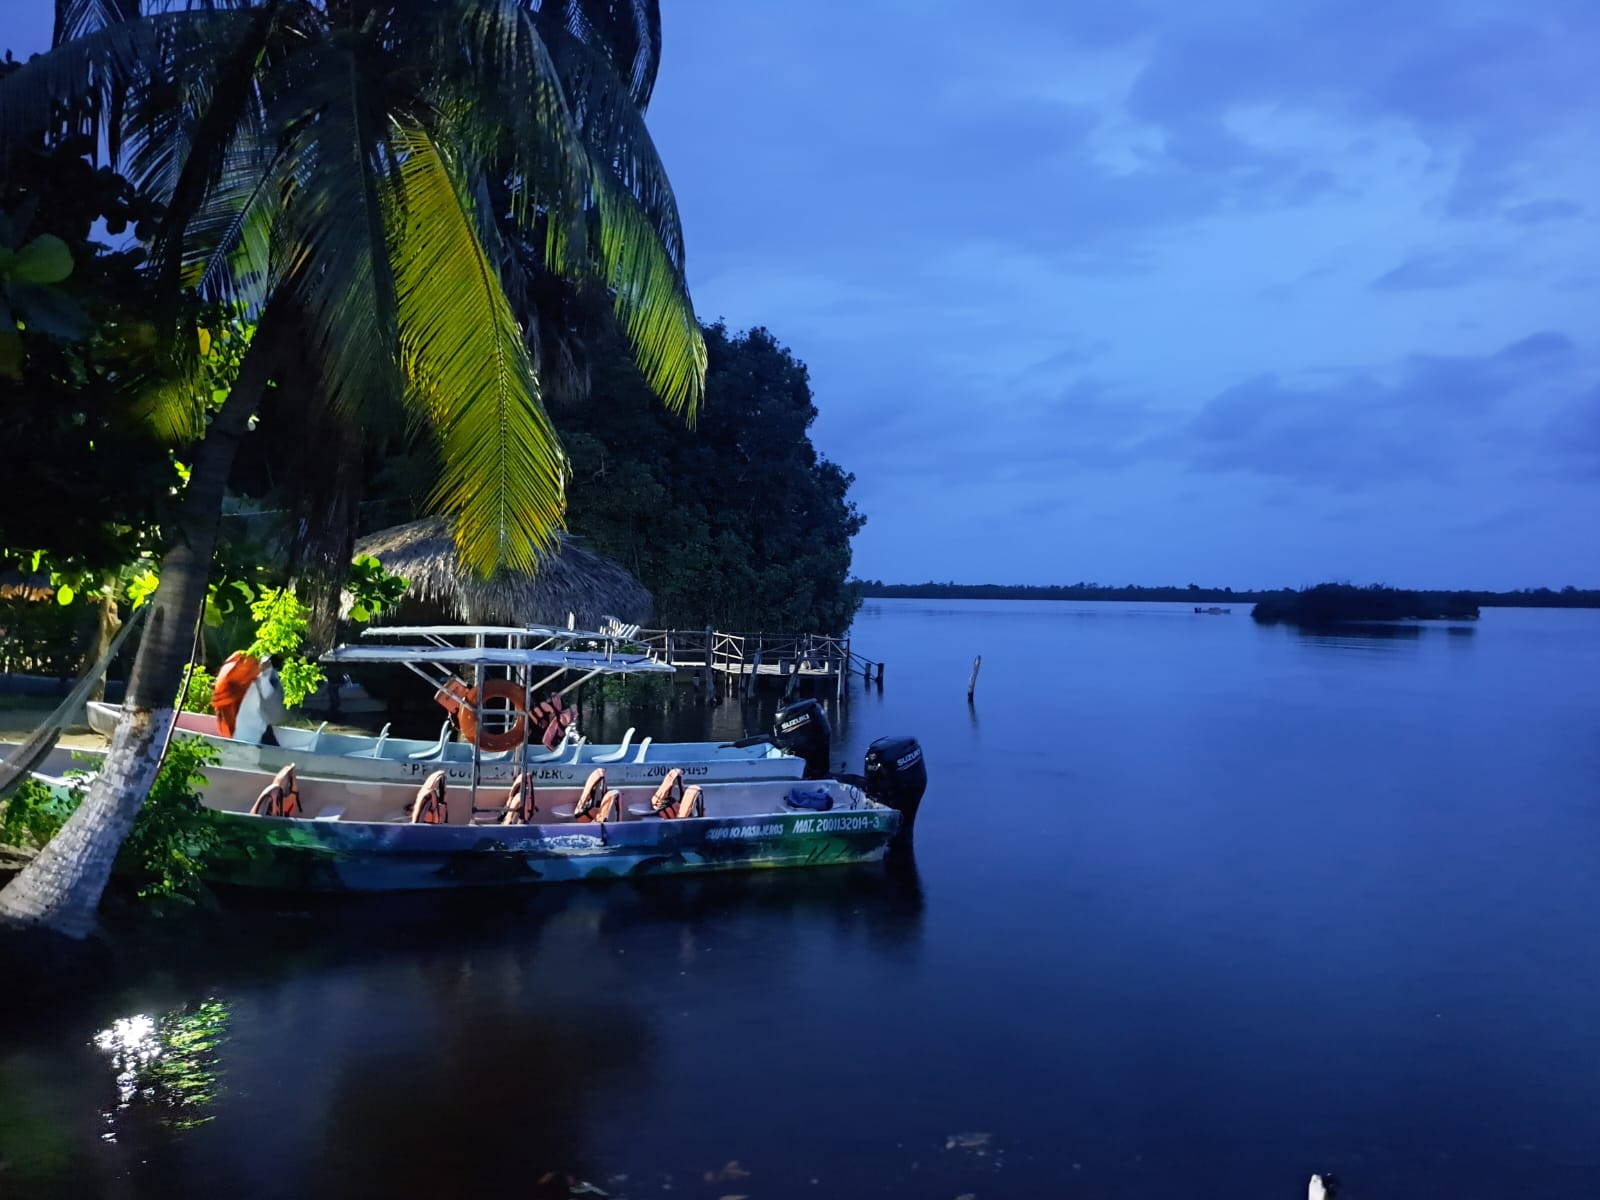
\includegraphics[width=\textwidth]{lago.jpeg}
        \caption*{\textbf{(a)}} % Pie de foto vacío, pero con la etiqueta
        \label{fig:sub1}
      \end{subfigure}\hspace{0.22cm}
      \begin{subfigure}[b]{0.22\textwidth}
        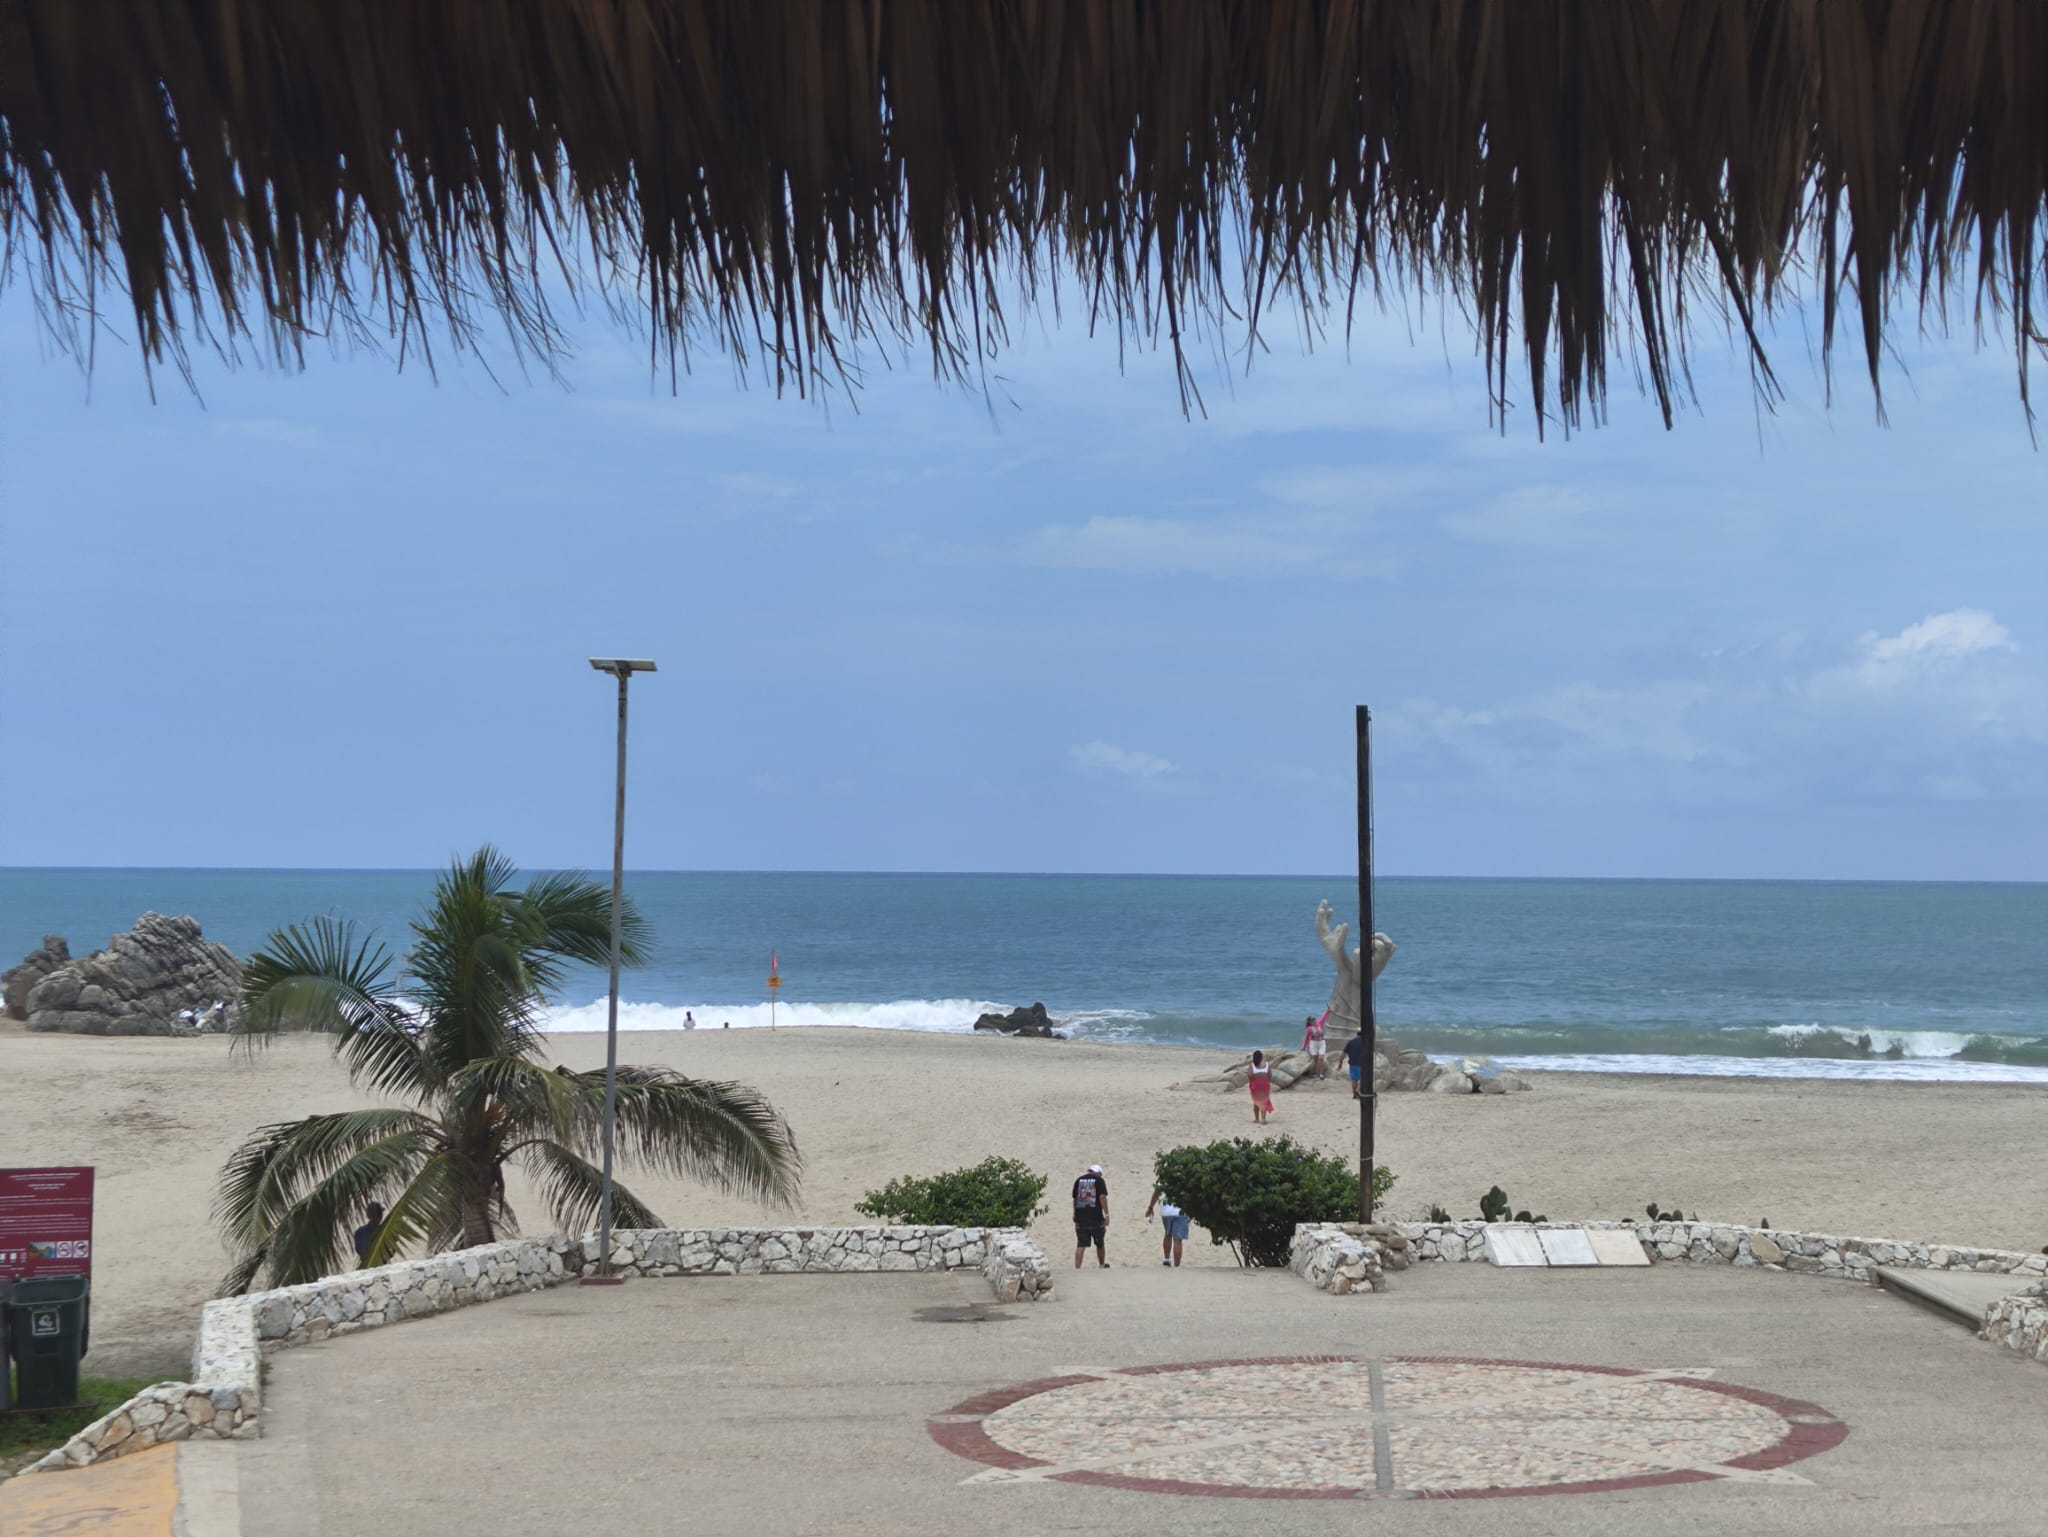
\includegraphics[width=\textwidth]{mar.jpeg}
        \caption*{\textbf{(b)}} % Pie de foto vacío, pero con la etiqueta
        \label{fig:sub2}
      \end{subfigure}

      \vspace{\baselineskip}

      \begin{subfigure}[b]{0.22\textwidth}
        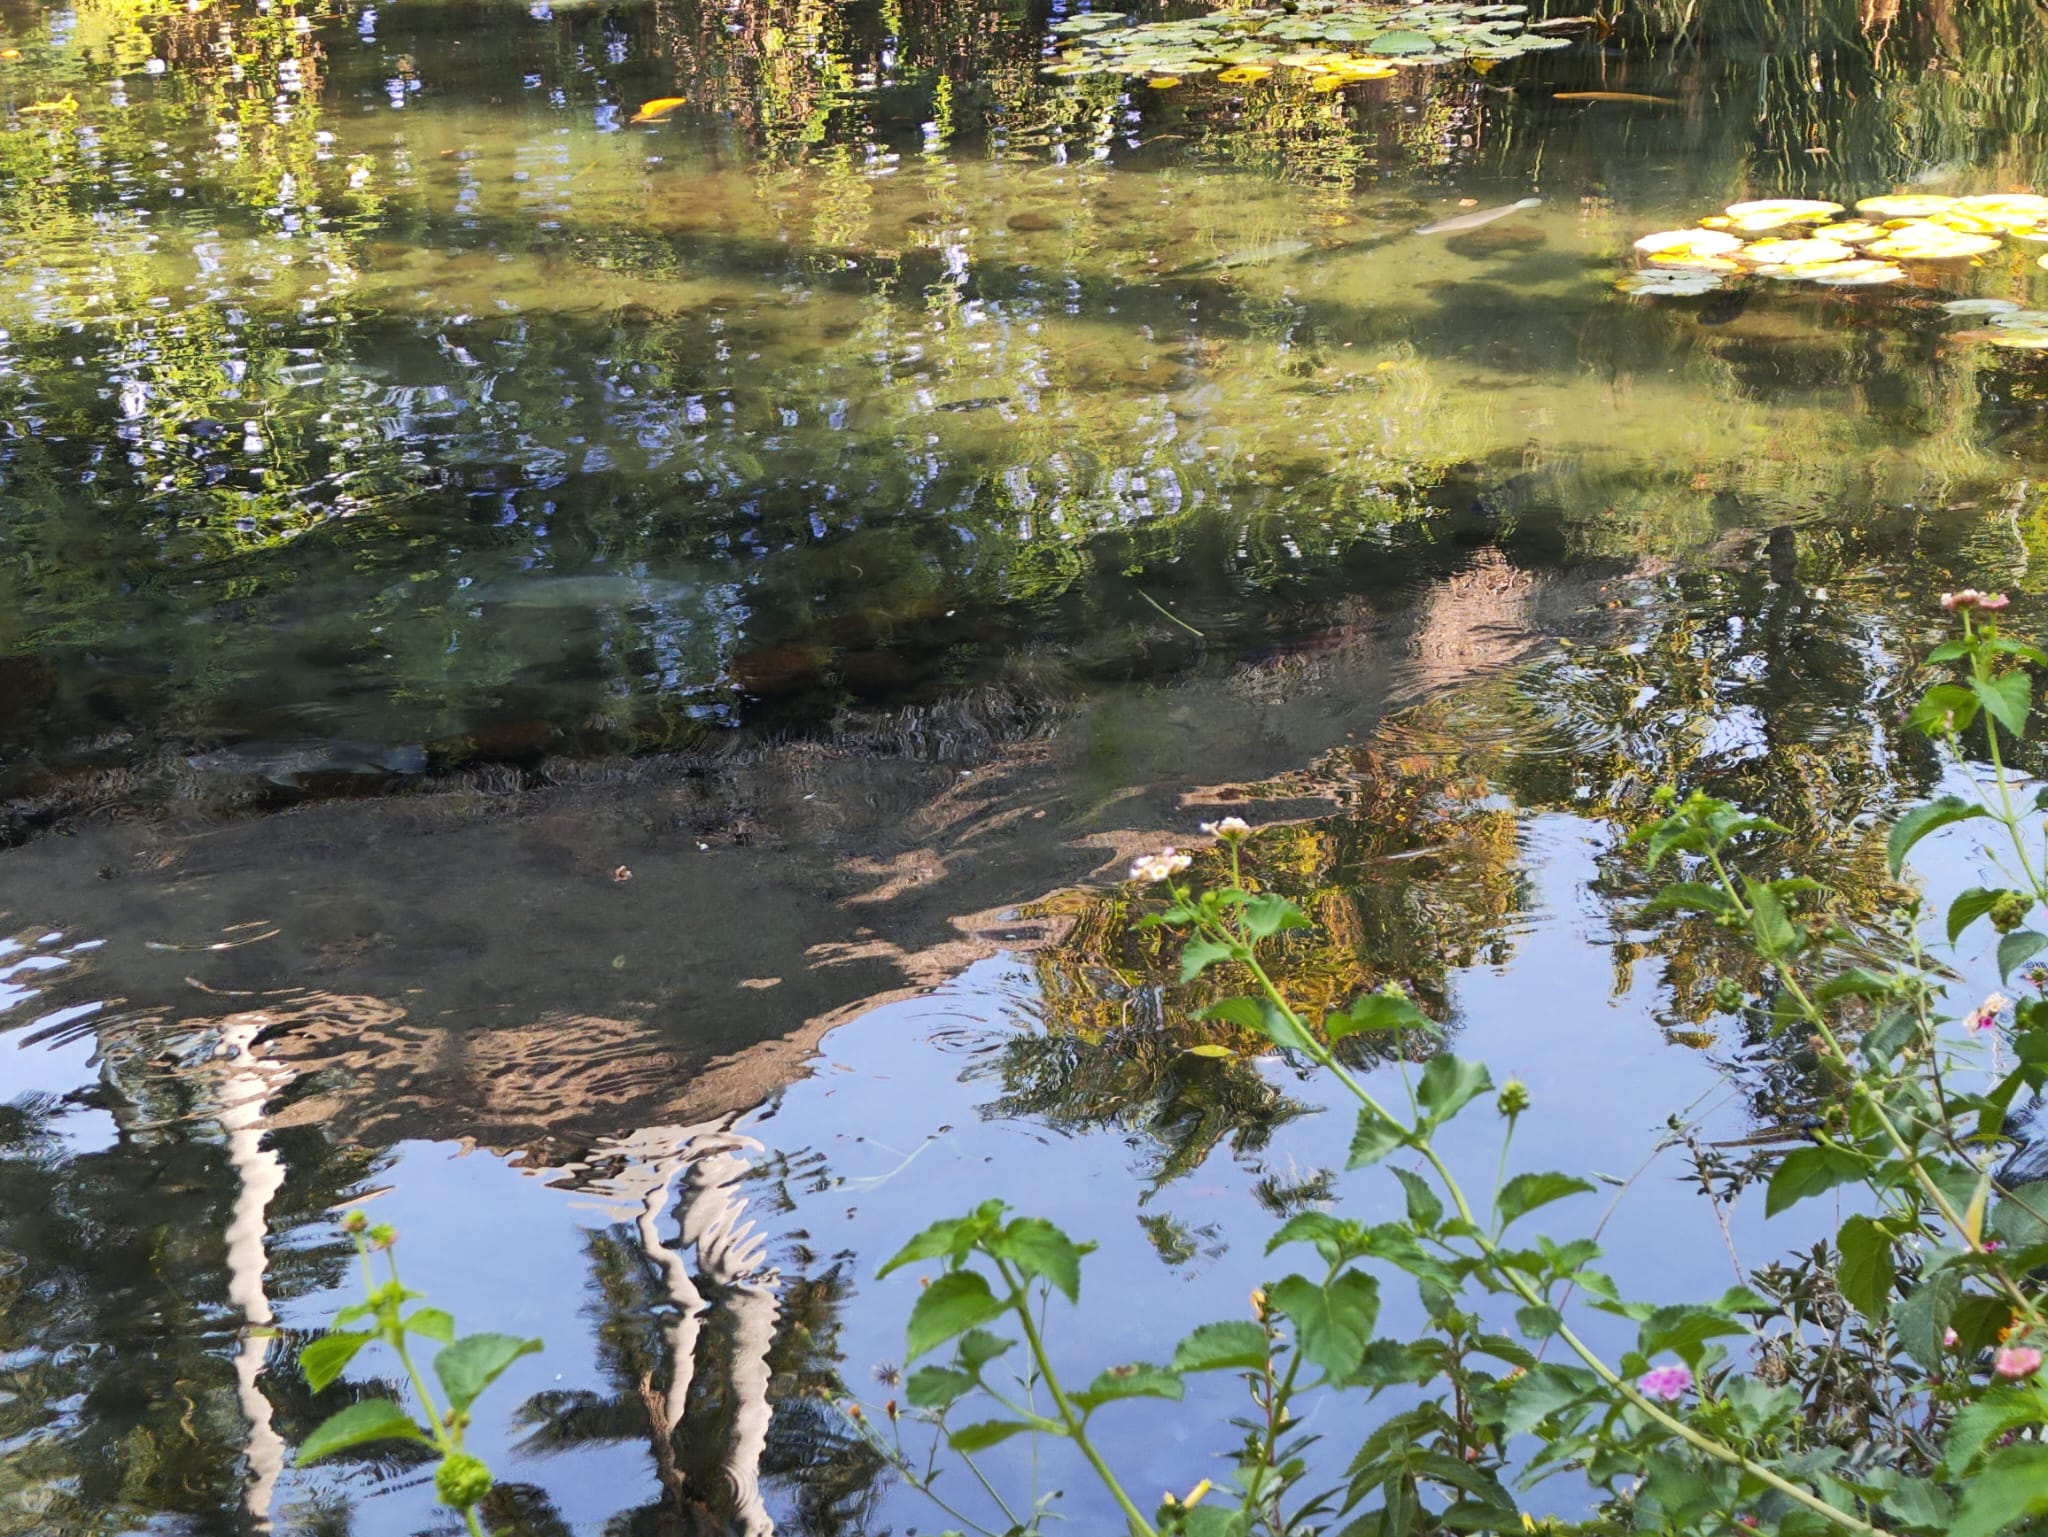
\includegraphics[width=\textwidth, height=2.2cm]{lodo.jpeg}
        \caption*{\textbf{(c)}} % Pie de foto vacío, pero con la etiqueta
        \label{fig:sub3}
      \end{subfigure}\hspace{0.5cm}
      \begin{subfigure}[b]{0.22\textwidth}
        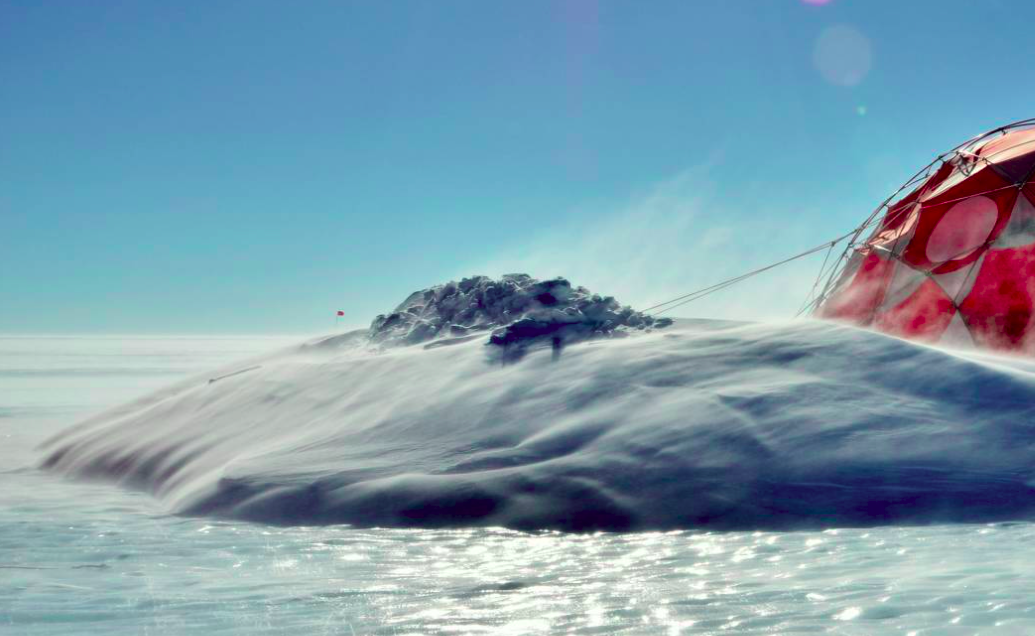
\includegraphics[width=\textwidth, height=2.2cm]{ice.png}
        \caption*{\textbf{(d)}} % Pie de foto vacío, pero con la etiqueta
        \label{fig:sub4}
      \end{subfigure}
       \captionsetup{labelformat=empty}
  \caption{\textbf{Figura 1:} Se han encontrado diatomeas en lagos \textbf{(a)} y mares \textbf{(b)}, en cuerpos de agua efímeros como tierra húmeda \textbf{(c)} e incluso en núcleos de hielo en la Antártica \textbf{(d)}.}

      \label{fig:cuatro_subfiguras}
    \end{figure}
\blfootnote{Fuente de la figura \textbf{(d)}: (Yan et al., 2019)}  
  }

\only<3>{
\vspace{0.7cm}
{Propiedades ecol\'ogicas de las diatomeas (Round et al., 1990): 

\vspace{0.4cm}

\begin{itemize}
%\item Organismos unicelulares fotosintéticos.
\item Grandes contribuyentes de oxígeno ($20-25\%$ del global).
\item Gran variedad de especies: más de 100,000 especies identificadas.
\item Valiosos indicadores históricos (debido a su acumulación).
\item Indicadores ambientales (debido a su variedad).
\item Parte esencial de la cadena alimenticia acuática.
\end{itemize}


}




}


\only<4>{
Las frústulas son un caparazón de sílice que aparece en la etapa de crecimiento del alga y establece una clasificación binaria dada por la simetría de las frústulas (Aguirre, et al., 2018).
   


}

\only<5>{

   \begin{figure}
      \centering
      \begin{subfigure}[b]{0.3\textwidth}
        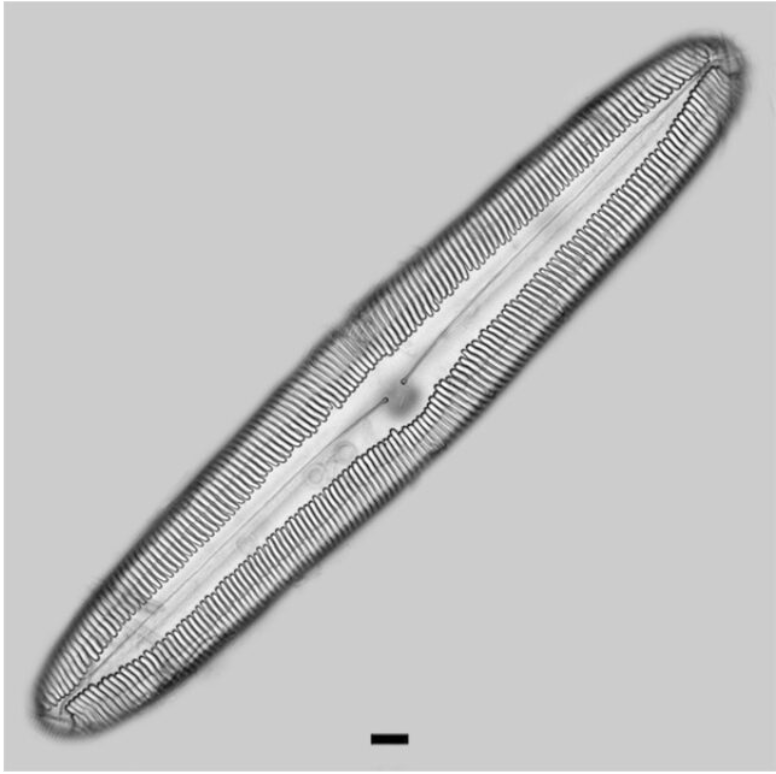
\includegraphics[width=\textwidth, height=2.2cm]{pen1.png}
        \caption*{\textbf{(a) \textit{Pinnularia dariana} }} % Pie de foto vacío, pero con la etiqueta
        \label{fig:sub1}
      \end{subfigure}\hspace{0.5cm}
      \begin{subfigure}[b]{0.3\textwidth}
        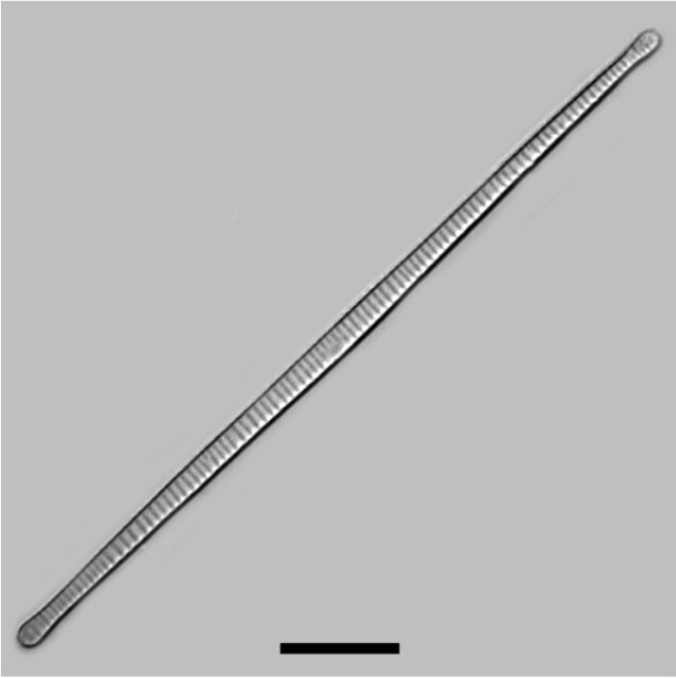
\includegraphics[width=\textwidth, height=2.2cm]{pen2.png}
        \caption*{\textbf{(b) \textit{Fragilaria synegrotesca}}} % Pie de foto vacío, pero con la etiqueta
        \label{fig:sub2}
      \end{subfigure}

      \vspace{\baselineskip}

      \begin{subfigure}[b]{0.3\textwidth}
        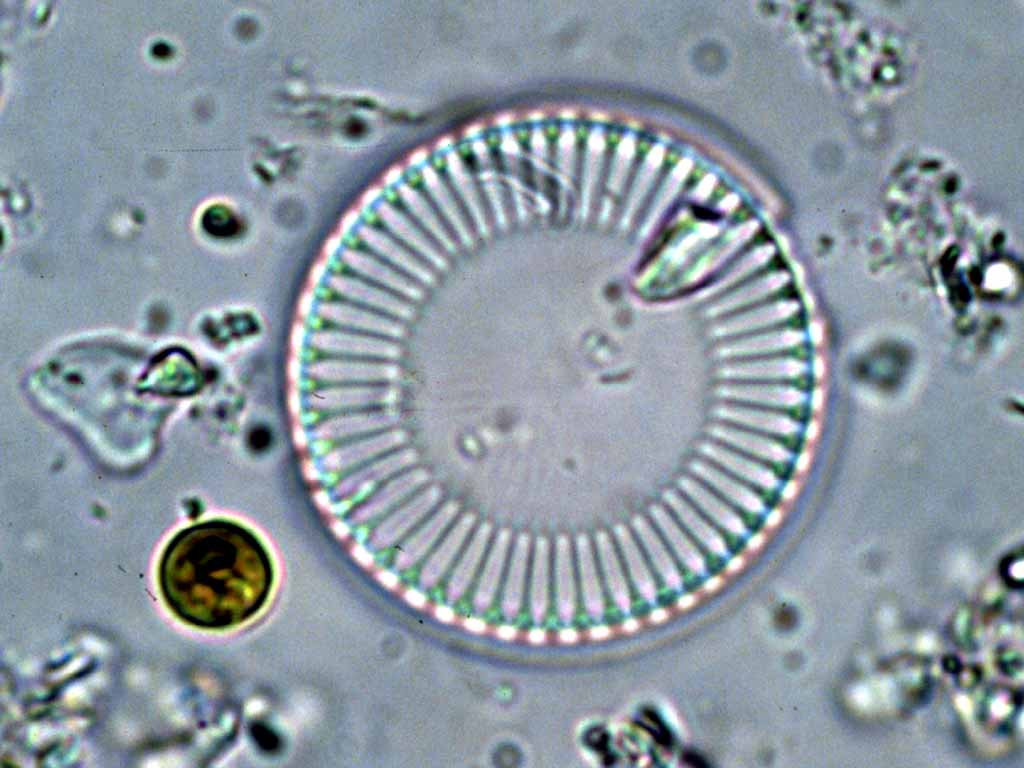
\includegraphics[width=\textwidth, height=2.2cm]{cen1.jpeg}
        \caption*{\textbf{(c) \textit{Cyclotella meneghiniana}}} % Pie de foto vacío, pero con la etiqueta
        \label{fig:sub3}
      \end{subfigure}\hspace{0.5cm}
      \begin{subfigure}[b]{0.3\textwidth}
        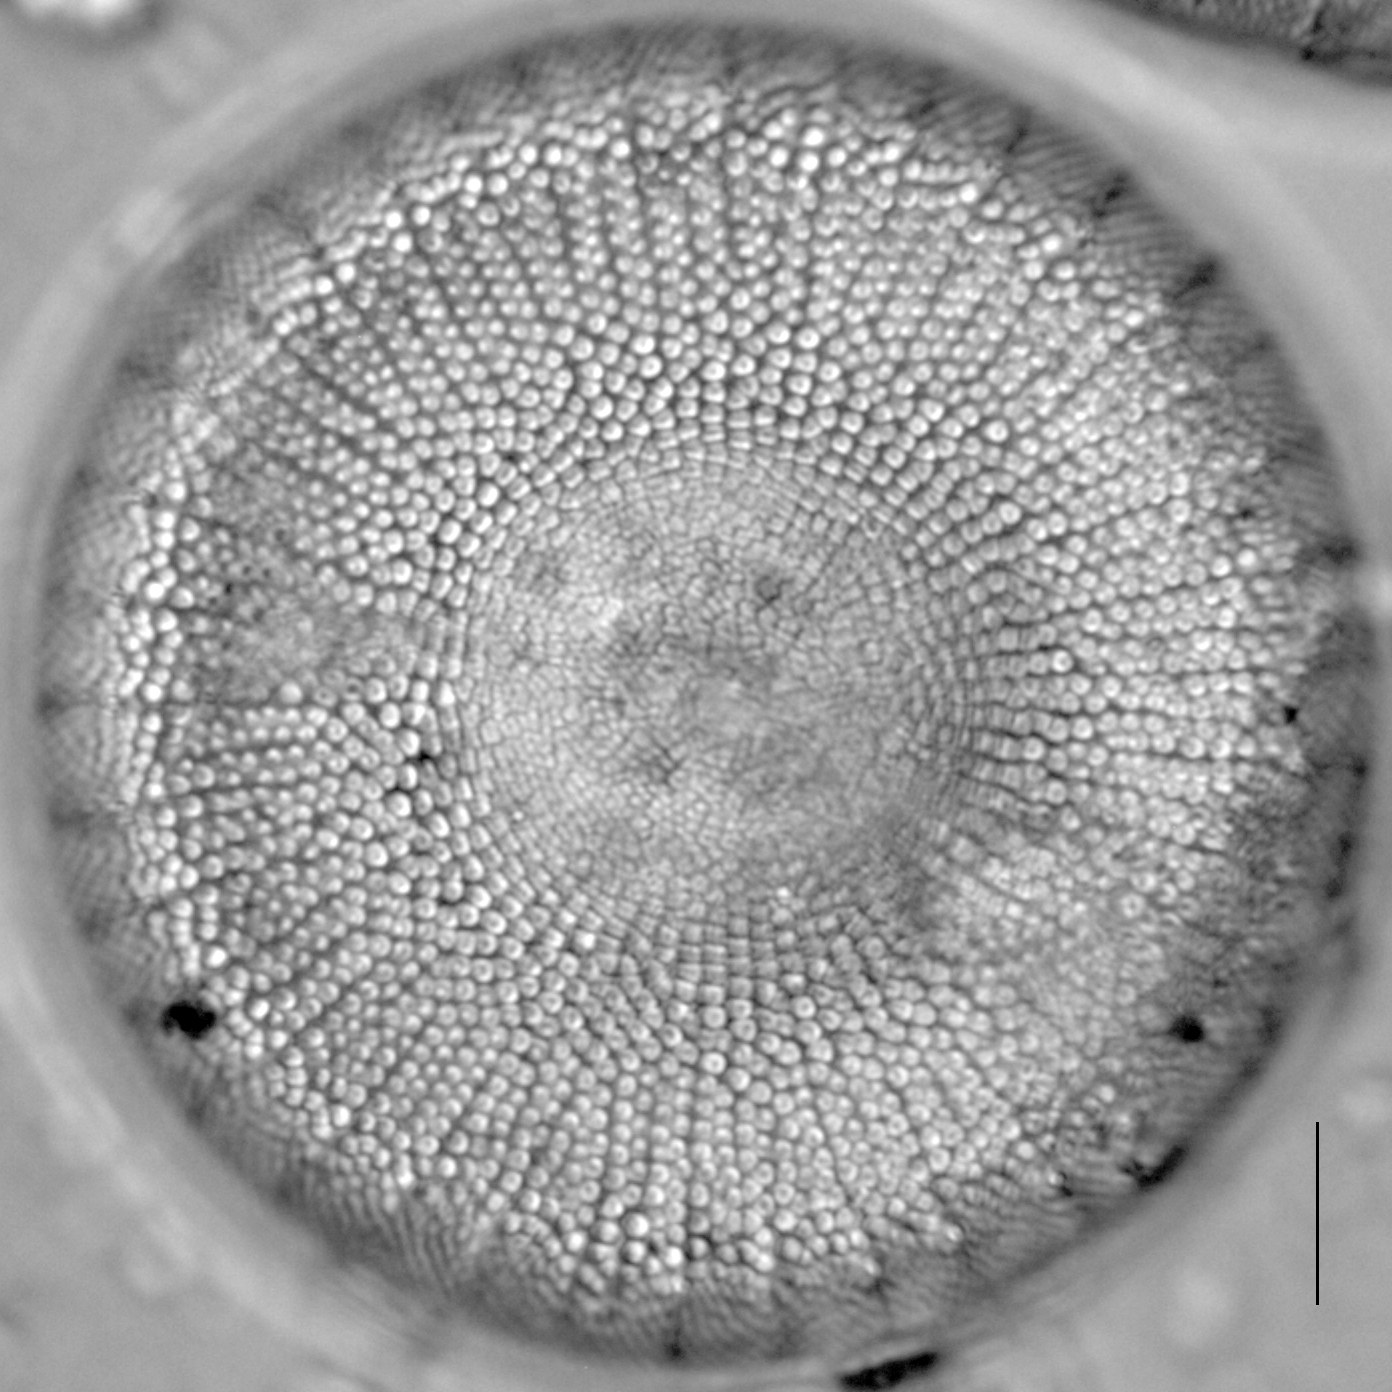
\includegraphics[width=\textwidth, height=2.2cm]{cen2.jpeg}
        \caption*{\textbf{(d) \textit{Stephanodiscus reimeri}}} % Pie de foto vacío, pero con la etiqueta
        \label{fig:sub4}
      \end{subfigure}
      \captionsetup{labelformat=empty}
  \caption{\textbf{Figura 2:} Ejemplos de diatomeas con simetrías bilateral y central. \textbf{(a-b)} Especies con simetría bilateral (diatomea pennada). \textbf{(c-d)} Especies con simetría central (diatomea céntrica).}
      \label{fig:cuatro2_subfiguras}
    \end{figure}
\blfootnote{Fuentes de las figuras:
    \textbf{(a):} (Pedreira, 2012), \textbf{(b-d):} (Diatoms of North America, 2023)}
}


\only<6>{
%Las frustulas tienen patrones intrensicos de poros y rendijas en toda su estructura. 

\begin{figure}
  \centering
  \begin{subfigure}[b]{0.2\linewidth}
    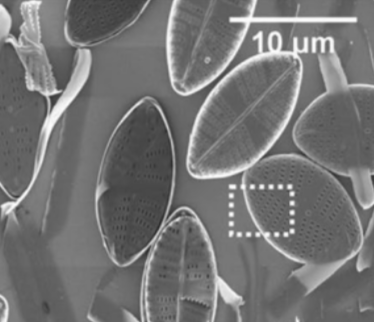
\includegraphics[width=0.9\linewidth]{Frustrulespictures/Screen Shot 2023-07-02 at 8.24.59 PM.png} % Renombra tu archivo a este
    \caption*{\textbf{(a)}}
    \label{fig7:a}
    %\vspace{0.1cm}
  \end{subfigure}\hspace{0.5cm} % Espacio horizontal de 0.5cm
  \begin{subfigure}[b]{0.2\linewidth}
    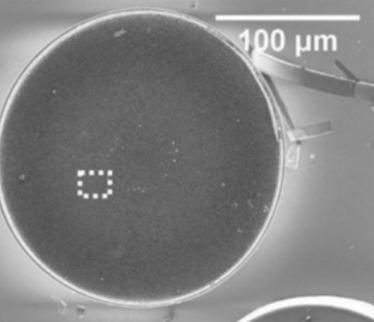
\includegraphics[width=0.9\linewidth]{Frustrulespictures/Screen Shot 2023-07-02 at 8.25.32 PM.png} % Renombra tu archivo a este
    \caption*{\textbf{(b)}}
    \label{fig7:b}
    %\vspace{0.2cm}
  \end{subfigure}

  \begin{subfigure}[b]{0.2\linewidth}
    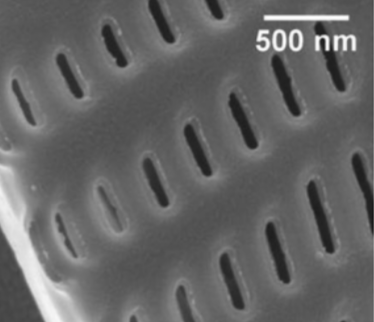
\includegraphics[width=0.9\linewidth]{Frustrulespictures/Screen Shot 2023-07-02 at 8.25.17 PM.png} % Renombra tu archivo a este
    \caption*{\textbf{(c)}}
    \label{fig7:c}
  \end{subfigure}\hspace{0.5cm} % Espacio horizontal de 0.5cm
  \begin{subfigure}[b]{0.2\linewidth}
    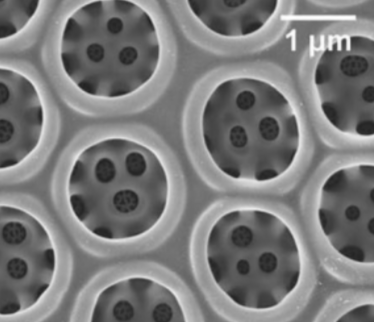
\includegraphics[width=0.9\linewidth]{Frustrulespictures/Screen Shot 2023-07-02 at 8.25.43 PM.png} % Renombra tu archivo a este
    \caption*{\textbf{(d)}}
    \label{fig7:d}
  \end{subfigure}
  \captionsetup{labelformat=empty}
  \caption{\textbf{Figura 3:}
Imágenes de microscopio electrónico de barrido (MEB) de \textbf{(a,c)} - \emph{Navicula perminuta}, \textbf{(b,d)} \emph{Coscinodiscus wailesii}. Los rectángulos punteados en \textbf{(a–b)} corresponden a las áreas magnificadas en \textbf{(c–d)} que exhibe la arquitectura del frústulo. }
  \label{poresfrustrules}
  

 
\end{figure}
\blfootnote{Fuente de las figuras \textbf{(a-d)}: (Aguirre et al., 2018)}

}



\only<7>{\begin{block}{Propiedades de las fr\'ustulas:}
\begin{itemize}
\item Las frústulas tienen patrones intrínsecos de poros y rendijas en toda su estructura.
\item Frústulo sintetizado a partir de ácido monosilícico.
\item El frústulo proporciona potencial protección UV.
\item El frústulo proporciona protección mecánica.
\item El frústulo exhibe estructuras similares a los cristales fot\'onicos.
\item Aplicaciones potenciales en la mejora de células solares.
\item Categorizadas por la simetría del frústulo (céntricas y pennadas).
\end{itemize}
\end{block}

\vspace{1cm}

}


\end{frame}



\begin{frame}{Marco teórico}{Microscopio invertido}

\begin{figure}
    \centering
    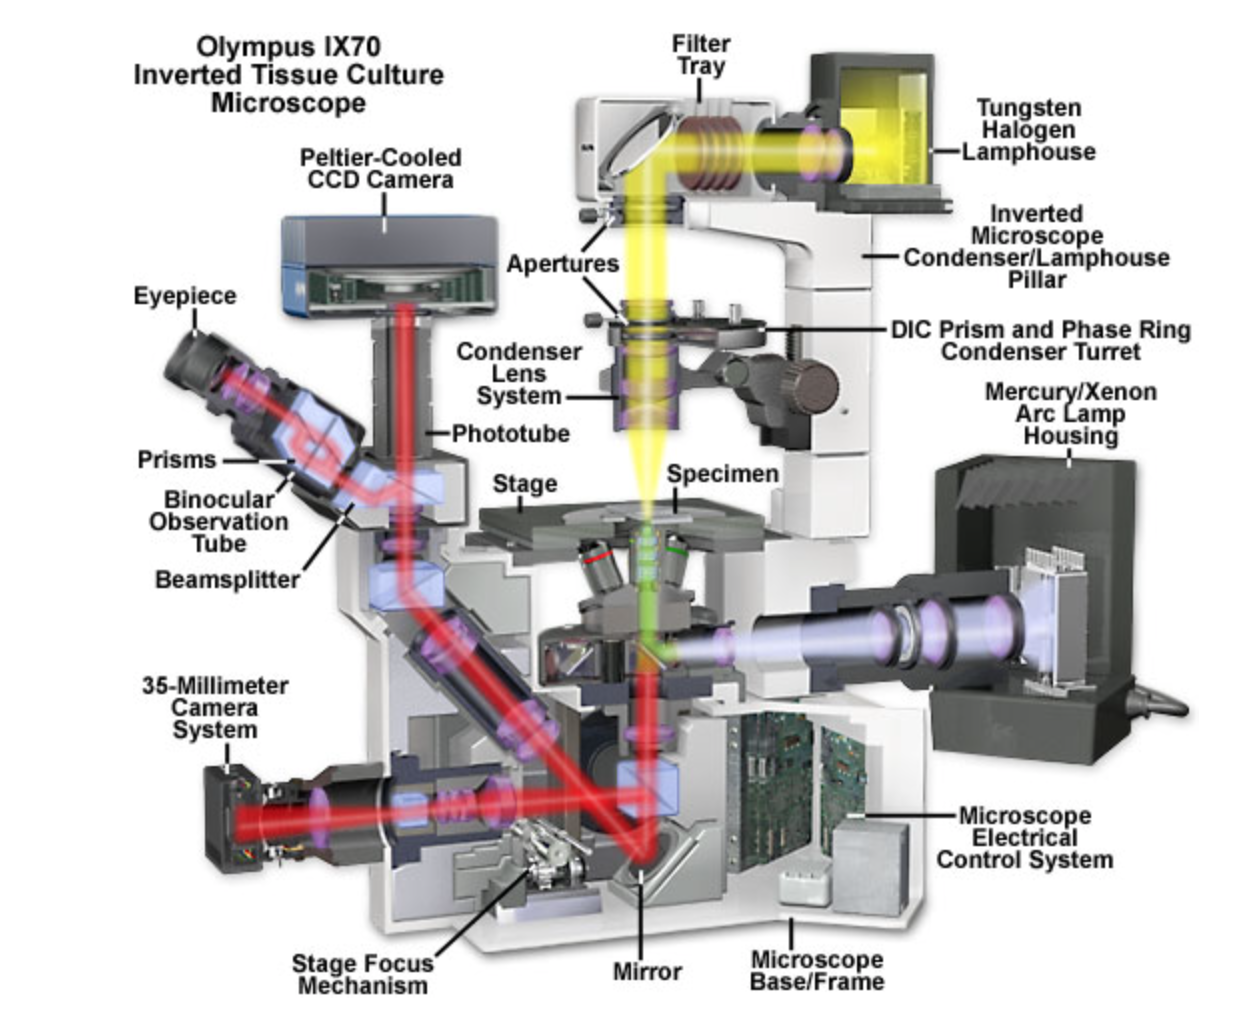
\includegraphics[scale=0.3]{Microscopeinvertedtrain.png}
    \captionsetup{labelformat=empty}
    \caption{\textbf{Figura 4:} Componentes de un microscopio invertido (microscopio Olympus IX70).}
    \label{Microscope inverted}
\end{figure}
\blfootnote{\scriptsize Fuente de la figura: (Fester et al., 2023)}


\end{frame}
%---------------------------------
\begin{frame}<1-10>
\frametitle{Marco teórico}


\framesubtitle{Pinzas ópticas}
\only<1>{
Las pinzas ópticas son dispositivos que permiten la manipulación sin contacto de objetos con tamaños que varían desde la escala atómica hasta la micrométrica.
\begin{block}{Pinzas ópticas}
\begin{itemize}
\item Consisten en un haz láser altamente enfocado.
\item Comúnmente, las pinzas ópticas se generan al enfocar el haz del láser sobrellenando una lente objetivo con un alto número de apertura numérica.
%\item Dependiendo de la relación entre la longitud de onda del láser y el tamaño de las partículas de estudio, se tienen regímenes teóricos para el estudio de las fuerzas que aparecen debido a la presión de radiación.
\end{itemize}





\end{block}}
%\only<2>{\frametitle{Marco teórico}\framesubtitle{Alineacion de las pinzas opticas.}
%$M_1$}
%$M_1$ y $M_2$}

\only<2>{\frametitle{Marco teórico}
\framesubtitle{Un modelo simple.}


\begin{figure}
    \centering
    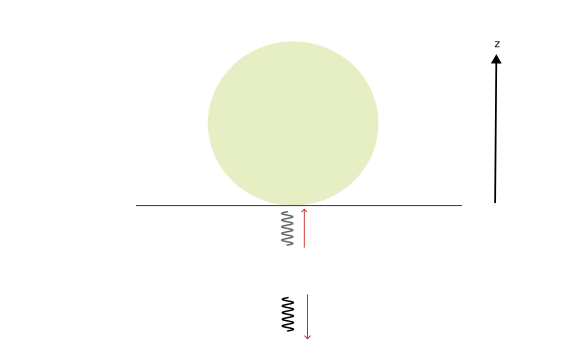
\includegraphics[scale=0.45]{foton2.png}
    \captionsetup{labelformat=empty}
    \caption{\textbf{Figura 5:} Un fot\'on con momento $\vec{p} = \frac{h}{\lambda} \hat{z}$ incide perpendicularmente en una part\'icula que funciona como un espejo perfecto.}
    \label{foton}
\end{figure}

}


\only<3>{\framesubtitle{Regímenes teóricos.}

El régimen teórico para aproximar el estudio de las fuerzas ópticas en las pinzas ópticas es determinado por (Jones et al., 2015)
\begin{equation}
\xi = \frac{2\pi a n_i}{\lambda_0}
\end{equation}
\vspace{0.8cm}
donde,
\begin{itemize}
    \item $\xi$ se define como el parámetro de tamaño de la partícula.
    \item $a$ es un parámetro característico del tamaño de la partícula.
    \item $\lambda_0$ representa la longitud de onda de la fuente de luz en el vacío, y
    \item $n_i$ es el índice de refracción del medio circundante.
\end{itemize}
}
\only<4>{
\begin{itemize}
    \item Si $\xi \gg 1$, el régimen de la óptica geométrica es una buena aproximación.
    \item Si $\xi \ll 1$, un tratamiento desde el punto de vista electromagnético (R\'egimen de Rayleigh) es adecuado, considerando a la partícula atrapada como un dipolo eléctrico inducido oscilante.
    \item Si $\xi \sim 1$, el régimen intermedio de la teoría generalizada de Lorenz-Mie es más adecuado para describir las fuerzas en las pinzas ópticas.
\end{itemize}
\vspace{0.8 cm}
En el caso de una partícula esférica de 10 micrómetros de radio en agua, siendo expuesta a un láser de $532 \, \text{nm}$ de longitud de onda, se tiene $\xi = 157.08 \gg 1$.
}



\only<5>{

\begin{figure}
    \centering
    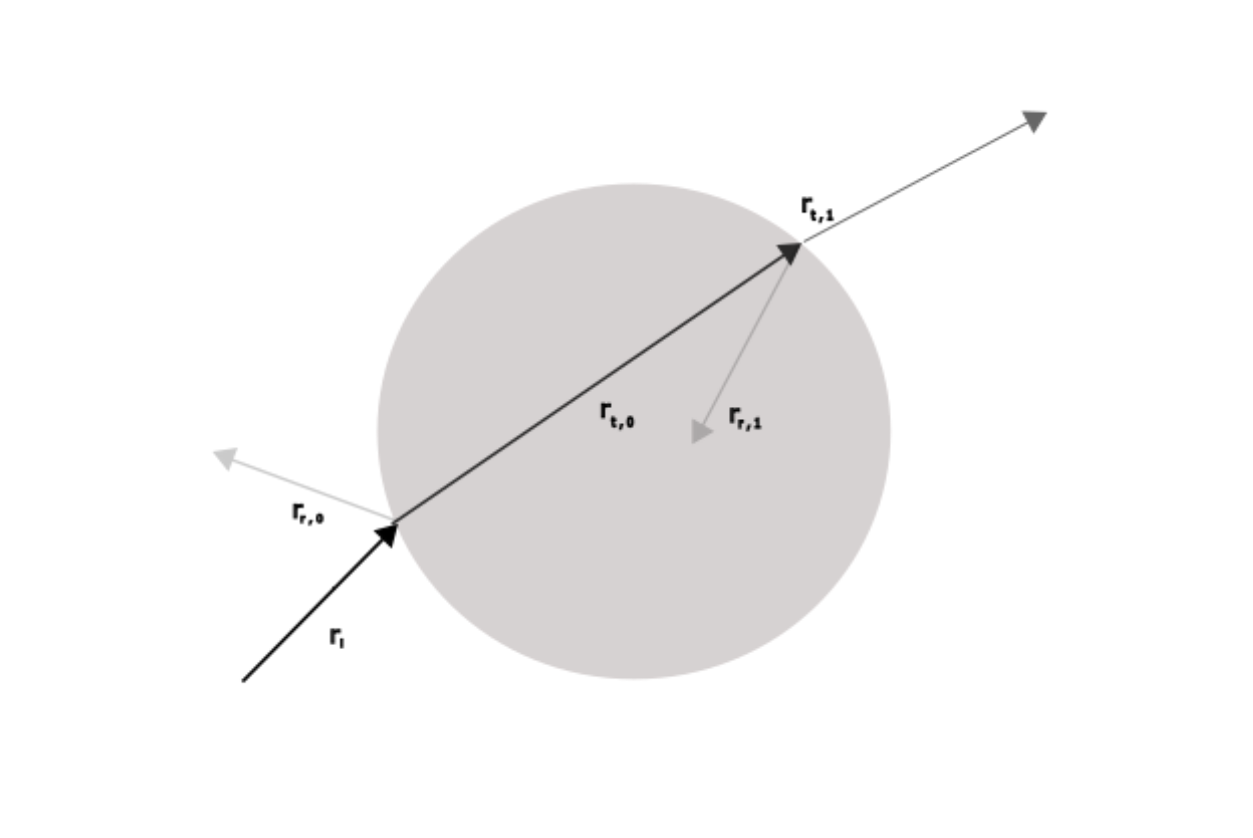
\includegraphics[scale=0.16]{beadrayoptics2.png}
    \captionsetup{labelformat=empty}
    \caption{\textbf{Figura 6:} Un rayo incidente $r_i$ incide sobre la superficie de una esfera. De esta interacción de dispersión, tendremos un componente transmitido y uno reflejado ($r_{r,0}$ y $r_{t,0}$) del rayo de luz. El rayo transmitido $r_{t,0}$ sufrirá otro proceso de dispersión, produciendo un nuevo par de haces de rayos ($r_{t,1}$ y $r_{r,1}$); el proceso de dispersión dentro de la esfera continuará hasta que toda la luz haya escapado de la esfera. Virtualmente toda la luz ha escapado de la esfera en menos de 10 eventos de dispersión.}
    \label{bead_optics}
\end{figure}
}



\only<6>{

\begin{figure}
    \centering
    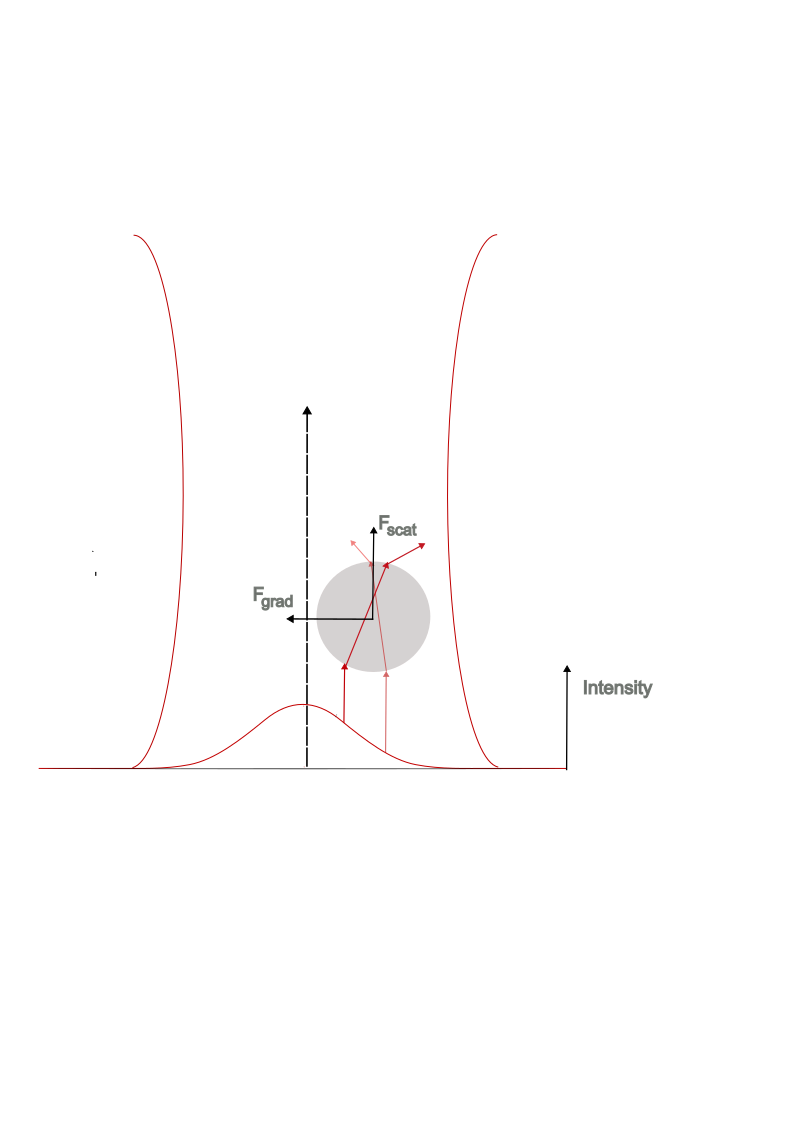
\includegraphics[trim={0cm 7.5cm 2cm 6cm },scale=0.37]{Imagenes teoria/Optical tweezer diagrams/finallyopticaltweezer.png}
    \captionsetup{labelformat=empty}
    \caption{\textbf{Figura 7:} Una part\'icula esferica sometida a un haz láser gaussiano. La esfera está fuera del eje de simetría del haz láser. Por lo tanto, la fuerza producida por el rayo de la izquierda será más fuerte que la del rayo de la derecha debido a un mayor número de fotones (mayor intensidad láser) para el primero. La figura muestra las fuerzas que actúan sobre la esfera debido al haz láser $F_{grad}$ y $F_{scat}$. }
    \label{Microscope inverted}
\end{figure}




}
\only<7>{\framesubtitle{Fuerza del primer evento de dispersión.}
Para un rayo incidente como el mostrado en la Figura 6, en su primer proceso de dispersión se tiene
\begin{equation*} % Use equation* to suppress automatic numbering
  \tag{2} % Manually add your equation number
  \mathbf{F}_{\text {ray }, 0}=\frac{n_{\mathrm{i}} P_{\mathrm{i}}}{c} \hat{\mathbf{r}}_{\mathrm{i}}-\frac{n_{\mathrm{i}} P_{\mathrm{r}}}{c} \hat{\mathbf{r}}_{\mathrm{r}}-\frac{n_{\mathrm{t}} P_{\mathrm{t}}}{c} \hat{\mathbf{r}}_{\mathrm{t}},
  \label{forcefirstevent}
\end{equation*}

\begin{itemize}
    \item $P_r$, $P_t$, y $P_i$ son las potencias del componente reflejado, transmitido e incidente del proceso de dispersión,
    \item $n_i$ y $n_t$ denotan los índices de refracción del medio, y la partícula respectivamente,
    \item $\hat{\mathbf{r_i}}$, $\hat{\mathbf{r_r}}$, y $\hat{\mathbf{r_t}}$ son los vectores unitarios que representan la dirección de los componentes incidente, reflejado y transmitido para el primer proceso de dispersión del rayo de luz incidente en la esfera.
\end{itemize}
}



\only<8>{\framesubtitle{El proceso asint\'otico por rayo.}
De manera teórica para este rayo incidente, se tendran infinitos procesos de dispersión,
\begin{equation*}
  \tag{3}
  \mathbf{F}_{\text {ray }}=\frac{n_{\mathrm{i}} P_{\mathrm{i}}}{c} \hat{\mathbf{r}}_{\mathrm{i}}-\frac{n_{\mathrm{i}} P_{\mathrm{r}}}{c} \hat{\mathbf{r}}_{\mathrm{r}, 0}-\sum_{n=1}^{+\infty} \frac{n_{\mathrm{i}} P_{\mathrm{t}, n}}{c} \hat{\mathbf{r}}_{\mathrm{t}, n},
  \label{infinitesum}
\end{equation*}
En principio se tendría que calcular la suma infinita para encontrar la fuerza exacta, sin embargo la contribución más grande proviene de los dos primeros procesos y virtualmente la potencia se vuelve cero despues de las 10 iteraciones del proceso.


}
\only<9>{\framesubtitle{La fuerza total}

La fuerza total debido al la radiacion electromagnetica, considerando \textbf{"todos"} los rayos del haz laser. 


\begin{equation*}
\tag{4}
\mathbf{F}_{\mathrm{total}}=\sum_m \mathbf{F}_{\mathrm{ray}}^{(m)}=\sum_m\left[\frac{n_{\mathrm{i}} P_{\mathrm{i}}^{(m)}}{c} \hat{\mathbf{r}}_{\mathrm{i}}^{(m)}-\frac{n_{\mathrm{i}} P_{\mathrm{r}}^{(m)}}{c} \hat{\mathbf{r}}_{\mathrm{r}, 0}^{(m)}-\sum_{n=1}^{+\infty} \frac{n_{\mathrm{i}} P_{\mathrm{t}, n}^{(m)}}{c} \hat{\mathbf{r}}_{\mathrm{t}, n}^{(m)}\right]. 
\label{Ftotal}
\end{equation*}


}
\only<10>{

\begin{figure}
    \centering
    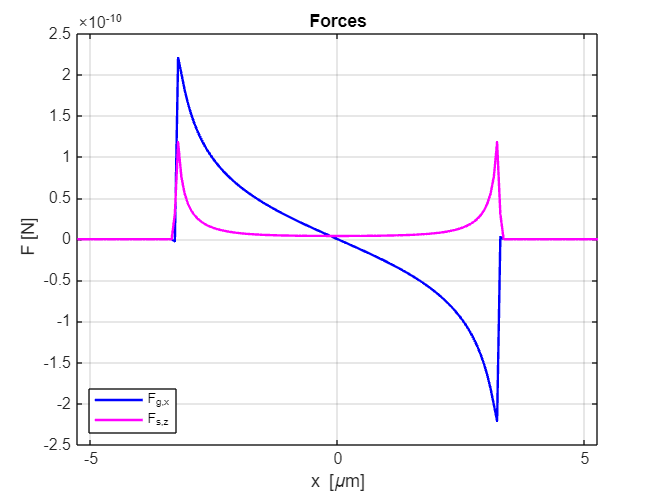
\includegraphics[scale=0.35]{Screenshot 2025-03-05 004832.png}
    \captionsetup{labelformat=empty}
    \caption{\textbf{Figura 8:} Fuerzas ópticas $F_g$ y $F_s$ (fuerza de gradiente y fuerza de dispersión respectivamente) sobre una partícula esférica de $SiO_2$ de $6.59 \mu m$ producidas por un haz láser enfocado con una potencia establecida en $120 mW$. Las fuerzas ópticas se calculan en función de la posición a lo largo del eje transversal x del centro de masa de la partícula atrapada utilizando el software OTGO (Callegari et al. (2015). El foco del haz láser en el software se considera obtenido sobrellenando un objetivo de microscopio con apertura numérica 1.0 y aumento de 60X.}
    \label{OpticalforcessetupKaren}
\end{figure} 

}


\end{frame}



\begin{frame}<1-4>
\frametitle{Marco teórico}
\only<1>{\frametitle{Marco teórico}\framesubtitle{Microfluidicos}
Un dispositivo microfluídico es un sistema diseñado para manipular y manejar pequeñas cantidades de fluidos a escala de micrómetros.
 \begin{figure}
     \centering
     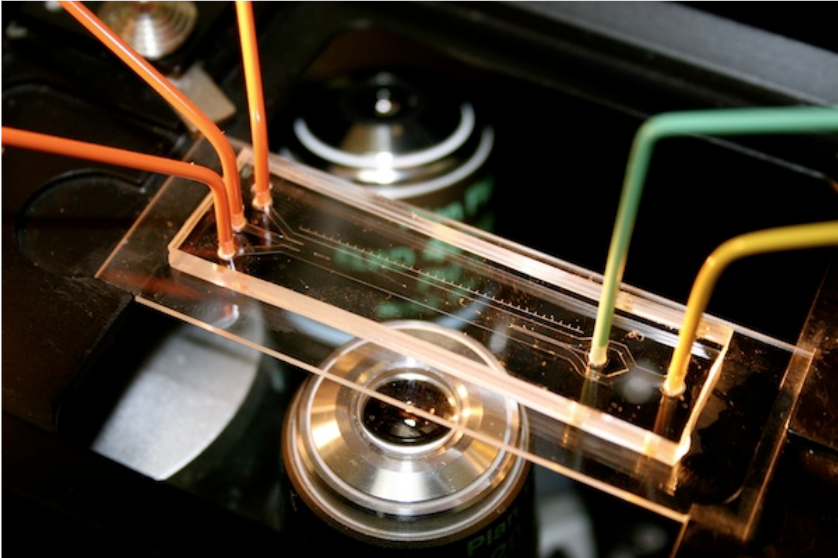
\includegraphics[scale=0.35]{microfluidicinaction.png}
     \captionsetup{labelformat = empty}
     \caption{\textbf{Figura 9:} Un dispositivo microfluídico colocado en la platina de un microscopio invertido. Esta configuración permite el seguimiento visual de los fenómenos que ocurren en los microcanales.}
     \label{microfluidic_device} .
 \end{figure}
\blfootnote{Fuente de la figura: (Wanucha ,2012)}}
 \only<2>{\framesubtitle{Microfluidicos: Un diseño simple.}
 
 \begin{figure}
     \centering
     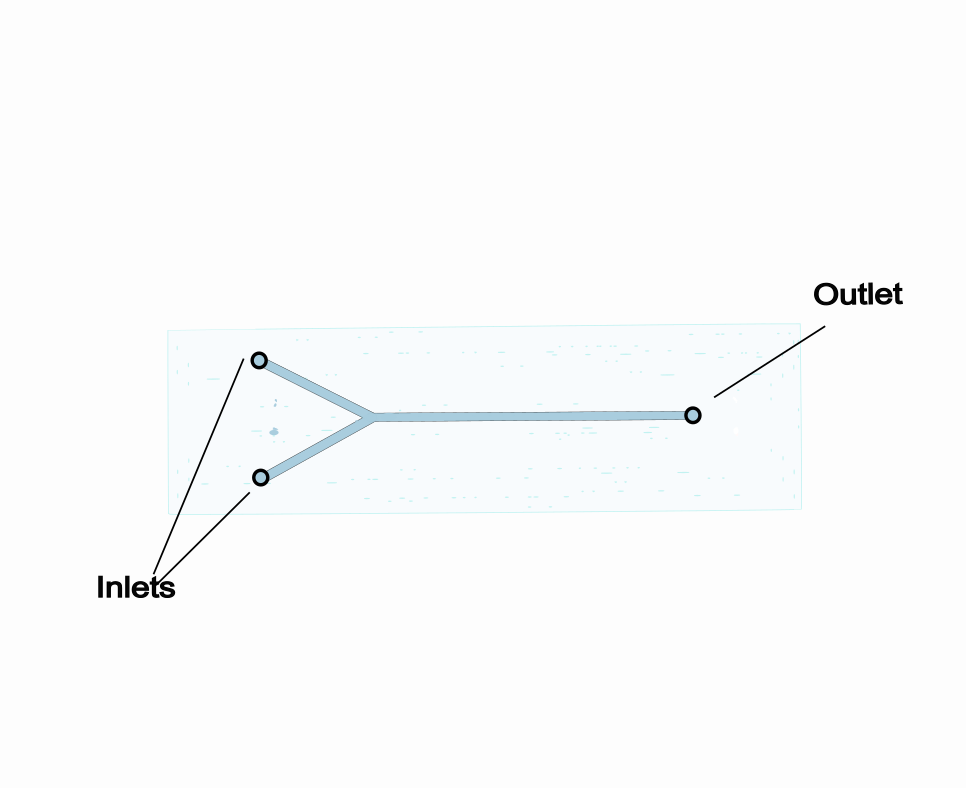
\includegraphics[trim = {0 1.5cm 0 0.7cm}, scale=0.4]{Diatomsexperimentalmethods/Microfluidics designs/Screen Shot 2024-01-17 at 5.34.18 PM.png}
     \captionsetup{labelformat = empty}
     \caption{\textbf{Figura 10:} Un diseño tipo Y de dispositivo microfluídico. Con dos entradas y una salida, este diseño es útil para aplicaciones de mezcla de microfluidos.}
     \label{simple design}
 \end{figure}
 
 
 
 }
\only<3>{\framesubtitle{Microfluidicos: propiedades}

 \begin{block}{Propiedades de los microfluidicos}
 \begin{itemize}
    \item Capacidad para manejar y manipular pequeñas cantidades de fluidos a escala de micrómetros o inferior.
    \item Red de microcanales interconectados.
    \item Control preciso del flujo del líquido.
    \item Permite un entorno estable para experimentos donde se requiere regulación estricta de temperatura, presión y concentraciones químicas.
    \item Proporciona un flujo continuo de fluído y recarga en caso de evaporación o intercambio de fluidos.
   % \item Permite la aceleración del fluído y la manipulación controlada.
    \item Fabricación con diversos materiales (silicio, vidrio, PDMS, metales).
    \item Variedad de diseños para la red de canales.
    \item Bajo consumo de muestra.
\end{itemize}
 \end{block}
 
 }
 
 \only<4>{\framesubtitle{La fuerza de Stokes}

Para una partícula esférica de radio \( r \) que se mueve con una velocidad \( \mathbf{v} \) en un fluído de viscosidad dinámica \( \mu \), la fuerza de arrastre \( \mathbf{F}_d \) es (Pau et al., 1990):
\begin{equation*}
\tag{5}
    \mathbf{F}_d = 6 \pi \mu r \mathbf{v}.
\end{equation*} 
 
 }
 
\end{frame}

\section{Métodos experimentales}
\begin{frame}{Métodos experimentales}{Arreglo experimental}

\begin{figure}
    \centering
    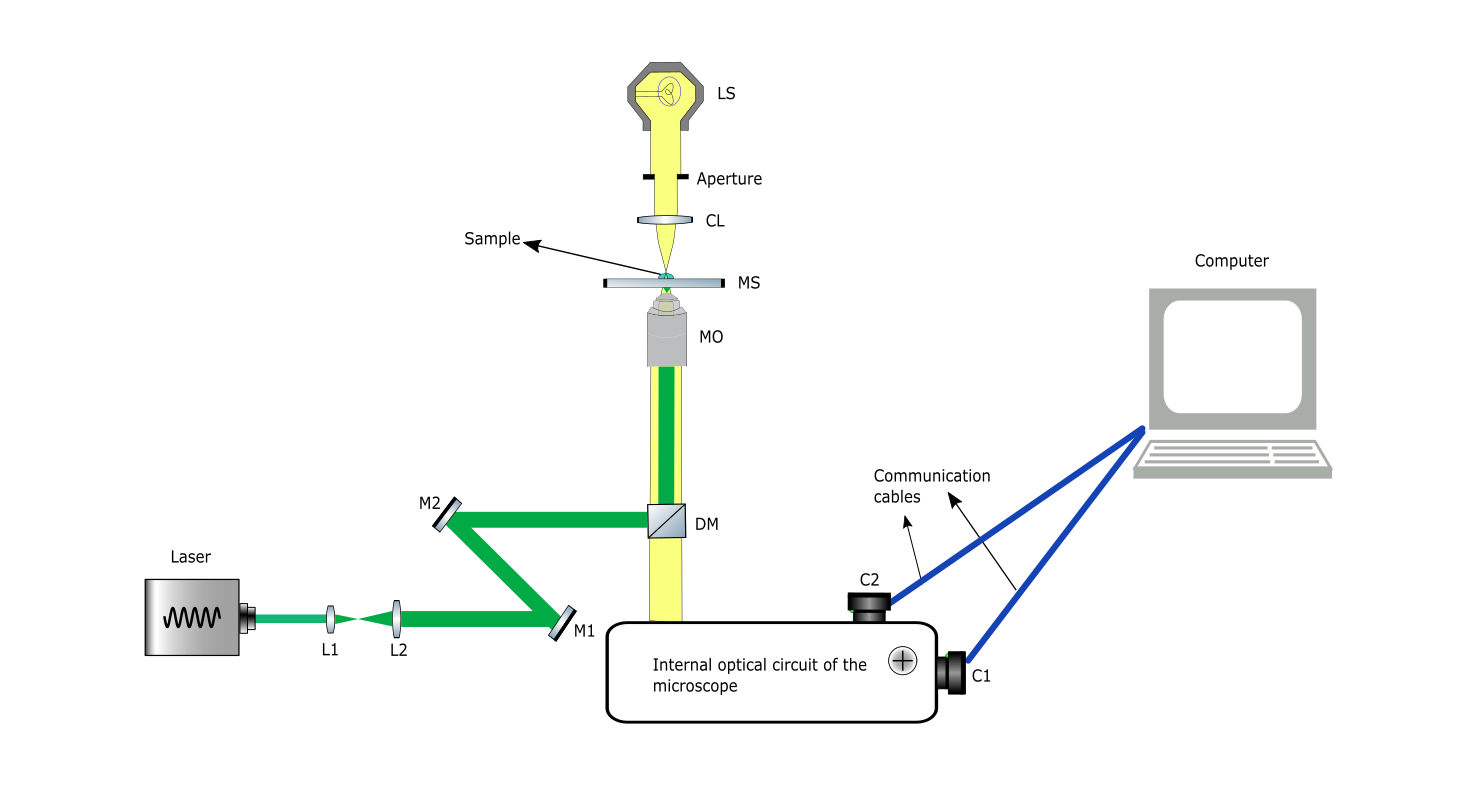
\includegraphics[scale=0.27]{Newplots_microfluidics_results/setup3.png}
    \captionsetup{labelformat = empty}
    \caption{\textbf{Figura 11:} Configuración estándar para pinzas ópticas. Un dispositivo láser facilita la radiación para producir la trampa óptica. $L_1$ y $L_2$ son dos lentes positivas. Estas lentes se colocan a una distancia $f_1 + f_2$ entre sí, expandiendo el haz láser para sobrellenar la apertura trasera del objetivo del microscopio (MO). $M_1$ y $M_2$ son espejos para alinear el haz láser. La luz láser es reflejada hacia la apertura trasera del objetivo del microscopio (MO) por un espejo dicróico (DM).}
    \label{setuptweezers}
\end{figure}

\end{frame}


\begin{frame}{Métodos experimentales}{Especificos}
\begin{itemize}
	\item Microscopio invertido Nikon Eclipse TE300
	\item 532 $nm$ Laser Quantum gem 532.
	\item Diferentes configuraciones de beam expanders (2x, 5x, y 10x).
	\item 60x objetivo de inmersi\'on de agua Nikon NA=1.00
	\item 100x objetivo de inmersi\'on de aceite Nikon NA=1.40
	\item Beam splitter CCM1-PBS25-532.
	\item NF533-17 filtros.
	\item AXIS M1103 C\'amaras.
	\item {Dispositivos microflu\'idicos de PDMS con canales de 100~\textmu m $\times$ 300~\textmu m.}
	\item CMA 4004 bomba externa para jeringa.
	

\end{itemize}
\end{frame}

\begin{frame}<1-4>\frametitle{Métodos experimentales}\framesubtitle{Muestras}
\only<1>{
\begin{itemize}
\item Las partículas de $SiO_2$ artificiales utilizadas ($24.82 \mu m$, $19.98 \mu m$, $6.59 \mu m$, y $4.27 \mu m$) estaban contenidas en una suspension acuosa con concentración de $2.5 \%$ peso/volumen.
\item Solución acuosa de células de levadura al $2\%$ peso/volumen.
\item Las especies de diatomeas utilizadas son \textit{Nitzschia sp}, \textit{Phaeodactylum tricornutum}, \textit{Thalassiosira pseudonana}, \textit{Navicula Sp. 12} y  \textit{Marine pennada}.
\end{itemize}




}


\only<2>{

\begin{figure} [H]
\centering
\begin{tabular}{ccc}
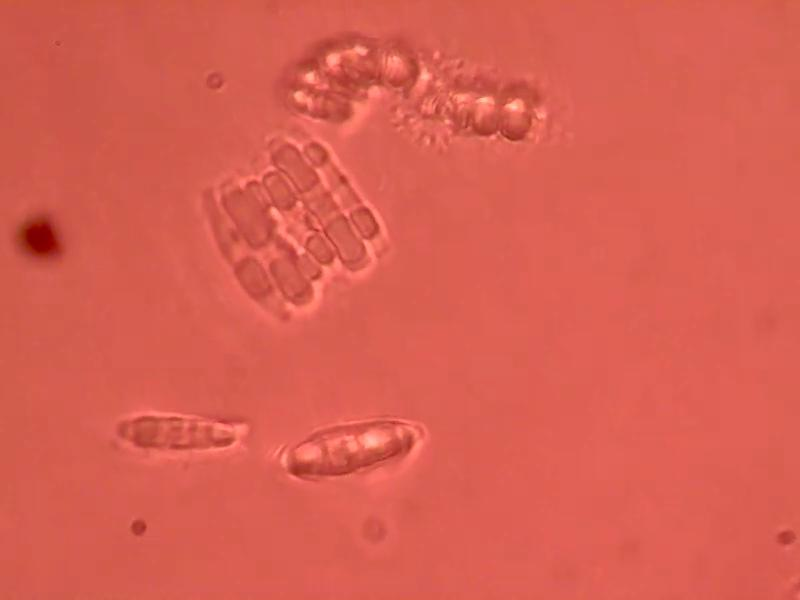
\includegraphics[width=0.22\textwidth]{Diatomsexperimentalmethods/Nitzchia sp1.jpeg} &
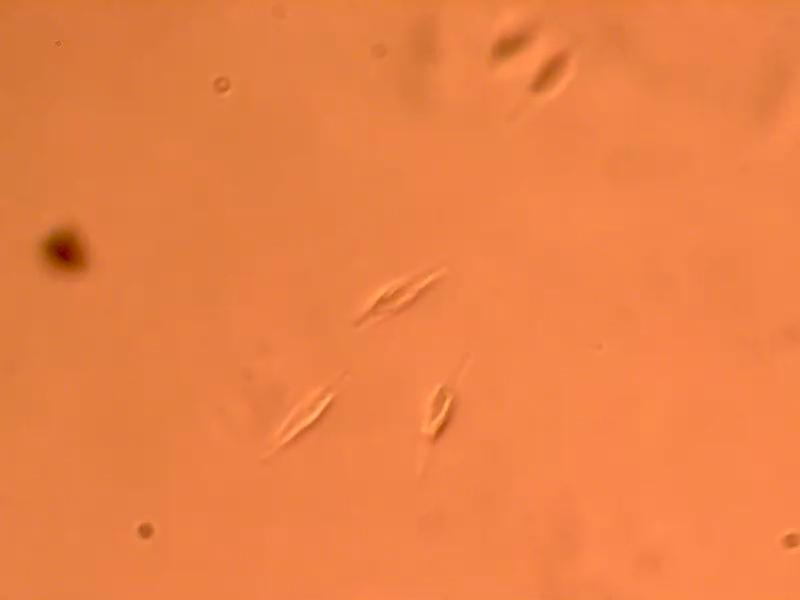
\includegraphics[width=0.22\textwidth]{Diatomsexperimentalmethods/Phaeodactylum t.jpgss.jpg} &
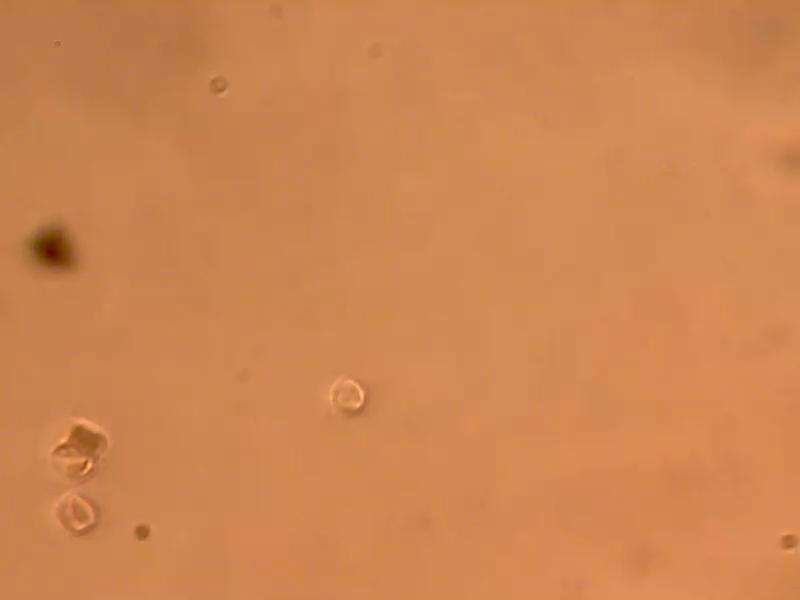
\includegraphics[width=0.22\textwidth]{Diatomsexperimentalmethods/thala2.jpeg} \\
\text{(a)}  & \text{(b)} & \text{(c)}  \\[6pt]
\end{tabular}

\vspace{6pt}

\begin{tabular}{cc}
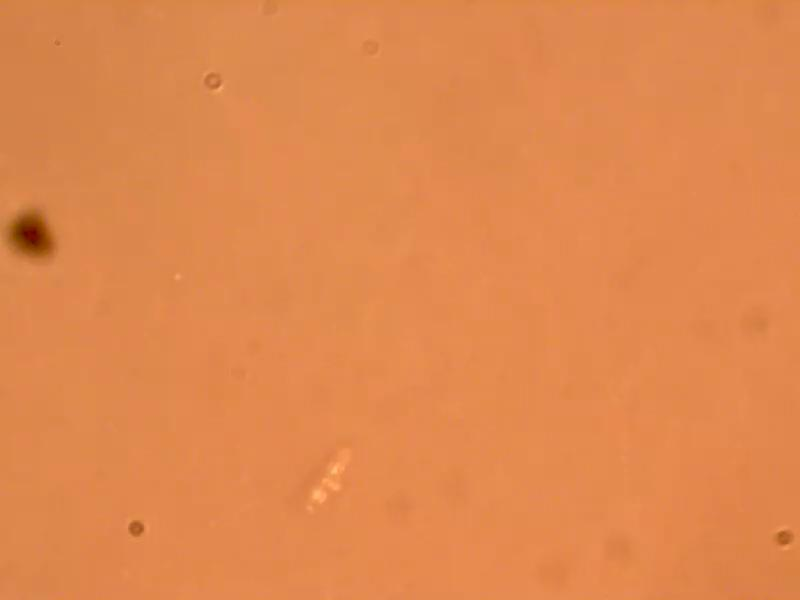
\includegraphics[width=0.22\textwidth]{Diatomsexperimentalmethods/gea4al.jpeg} &
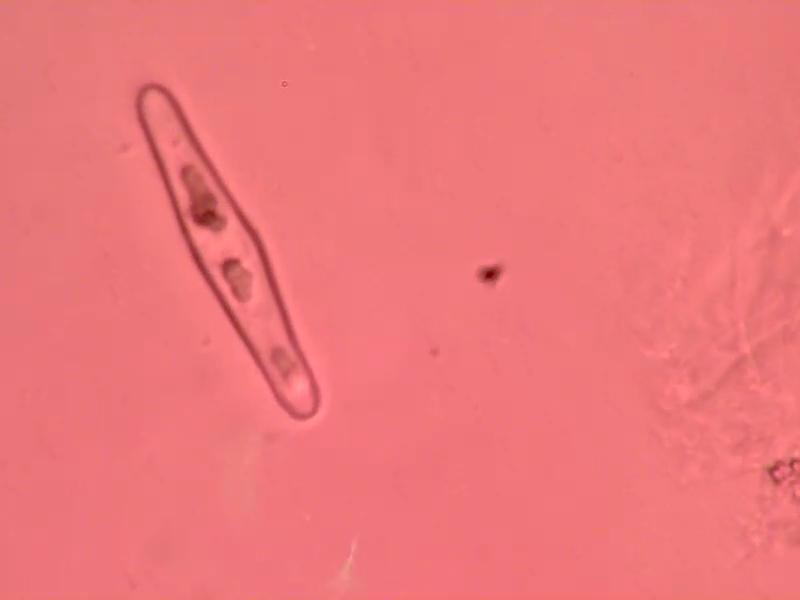
\includegraphics[width=0.22\textwidth]{Diatomsexperimentalmethods/ray.jpeg} \\
\text{(d)}  & \text{(e)}  \\[6pt]
\end{tabular}
\captionsetup{labelformat=empty}
\caption{\textbf{Figura 12:} Especies de diatomeas estudiadas en este trabajo, fotografiadas con el objetivo de microscopio de inmersión en agua. (a) Multitud de \textit{Nitzschia sp}. (b) muestra de la especie de diatomea \textit{Phaeodactylum tricornutum}. (c) muestra de la especie de diatomea \textit{Thalassiosira pseudonana}. (d) Diatomea \textit{Navicula Sp. 12}. (e) Diatomea \textit{Pennada marina}}.
\label{DiatomExperiments}
\end{figure}



}

\only<3>{\framesubtitle{Preparación de muestras}

\begin{figure}
    \centering
    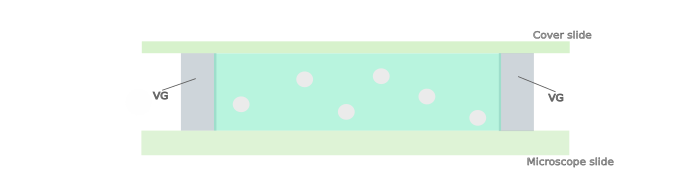
\includegraphics[trim ={1cm 0 0cm 0cm}, scale=.6]{Imagenes teoria/cuci.png}
	\captionsetup{labelformat=empty}    
    \caption{\textbf{Figura 13}: Preparación de la muestra. Una barrera de grasa de vacío (VG) contiene las suspensiones acuosas con las partículas a ser atrapadas entre el cubreobjetos y el portaobjetos.} 
    \label{VG}
\end{figure}




}
\only<4>{
\framesubtitle{Microfluidicos}
\begin{figure}[H]
    \centering
    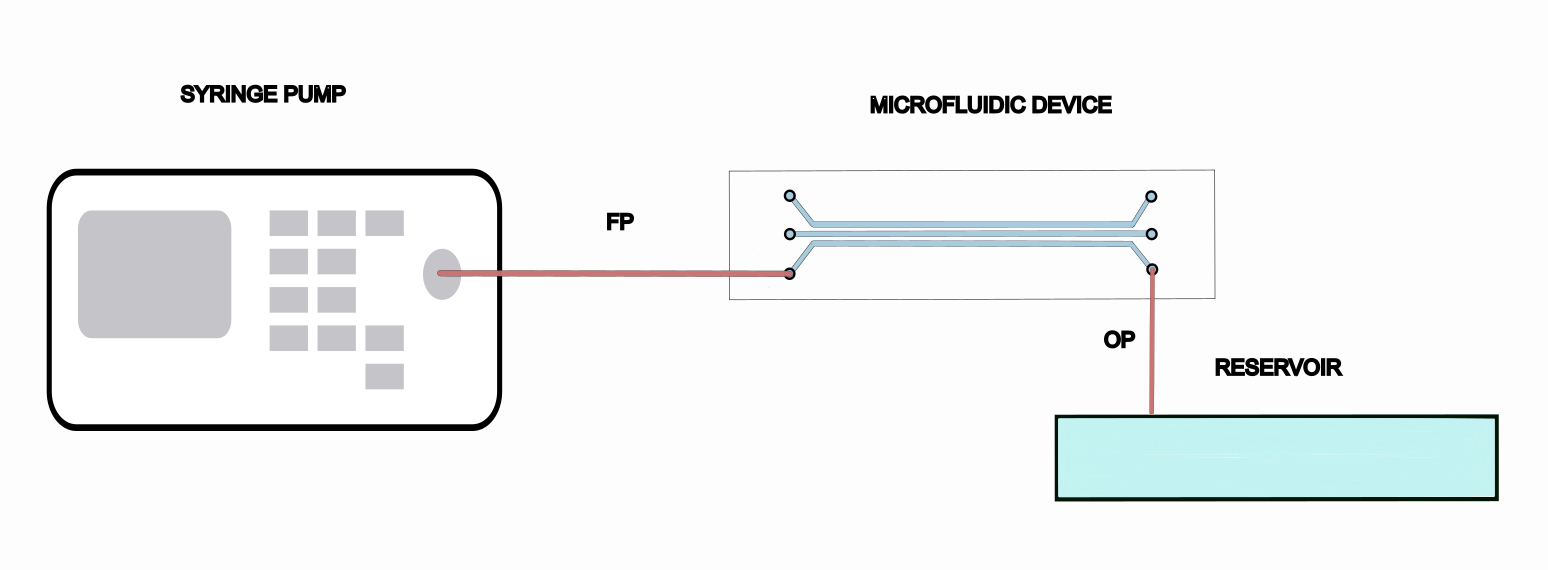
\includegraphics[scale=0.35]{Diatomsexperimentalmethods/Samplepreparation/Screen Shot 2024-01-18 at 12.50.20 PM.png}
    \captionsetup{labelformat=empty}
    \caption{\textbf{Figura 14:} Esquema del sistema microfluídico. La bomba de jeringa controla la velocidad de flujo de la solución que entra al canal a través del tubo de alimentación (FP) integrado en la entrada del canal. Una vez que el fluído alcanza la salida del canal, un tubo de salida (OP) dirige la solución efluente a un reservorio.}
    \label{microfluidicsystem}
\end{figure}


}

\end{frame}



%-------------------------------------------------------
\section{Resultados}
%-------------------------------------------------------
\begin{frame}
\frametitle{Resultados}\framesubtitle{Manipulacion de partículas de silica.}





\begin{figure}
    \centering
    \includemovie[autoplay]{12cm}{7cm}{video2.mp4}
    \captionsetup{labelformat=empty}
    \caption{\textbf{Figura 15:} Atrapamiento de partículas de $SiO_{2}$ de $6.59 \mu m$. La trampa se produjo con el objetivo de inmersión en agua (MO) y un expansor de haz de 2x (potencia láser establecida en 42 $mW$).}
    \label{fig:enter-label}
\end{figure}


\end{frame}

\begin{frame}<1-2>
\frametitle{Resultados}\framesubtitle{Atrapamiento de células de levadura.}
\only<1>{

\begin{figure}
  \centering
  \begin{subfigure}[b]{0.2\linewidth}
    \includegraphics[width=\linewidth ,height=2.3cm]{particles2.png} % Renombra tu archivo a este
    \caption*{\textbf{(a)}}
    \label{fig7:a}
    %\vspace{0.1cm}
  \end{subfigure}\hspace{0.5cm} % Espacio horizontal de 0.5cm
  \begin{subfigure}[b]{0.2\linewidth}
    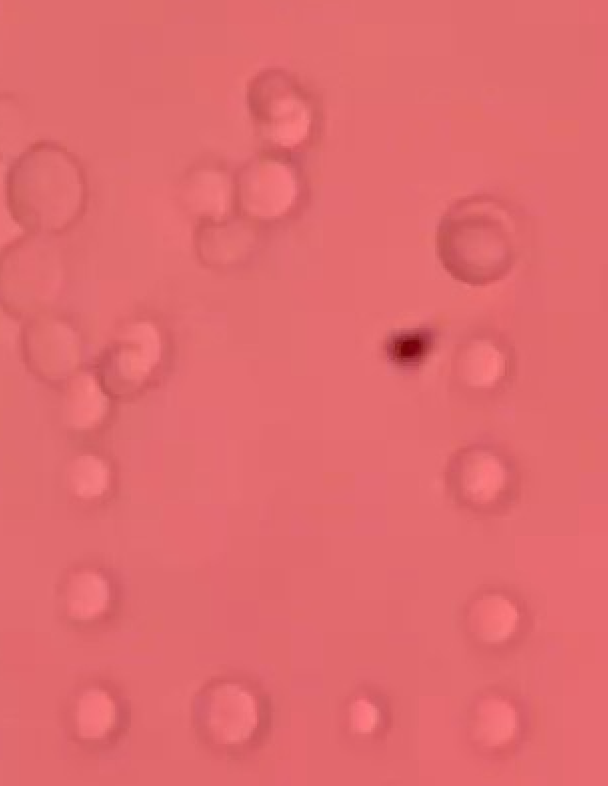
\includegraphics[width=\linewidth ,height=2.3cm]{particles7.png} % Renombra tu archivo a este
    \caption*{\textbf{(b)}}
    \label{fig7:b}
    %\vspace{0.2cm}
  \end{subfigure}

  \begin{subfigure}[b]{0.2\linewidth}
    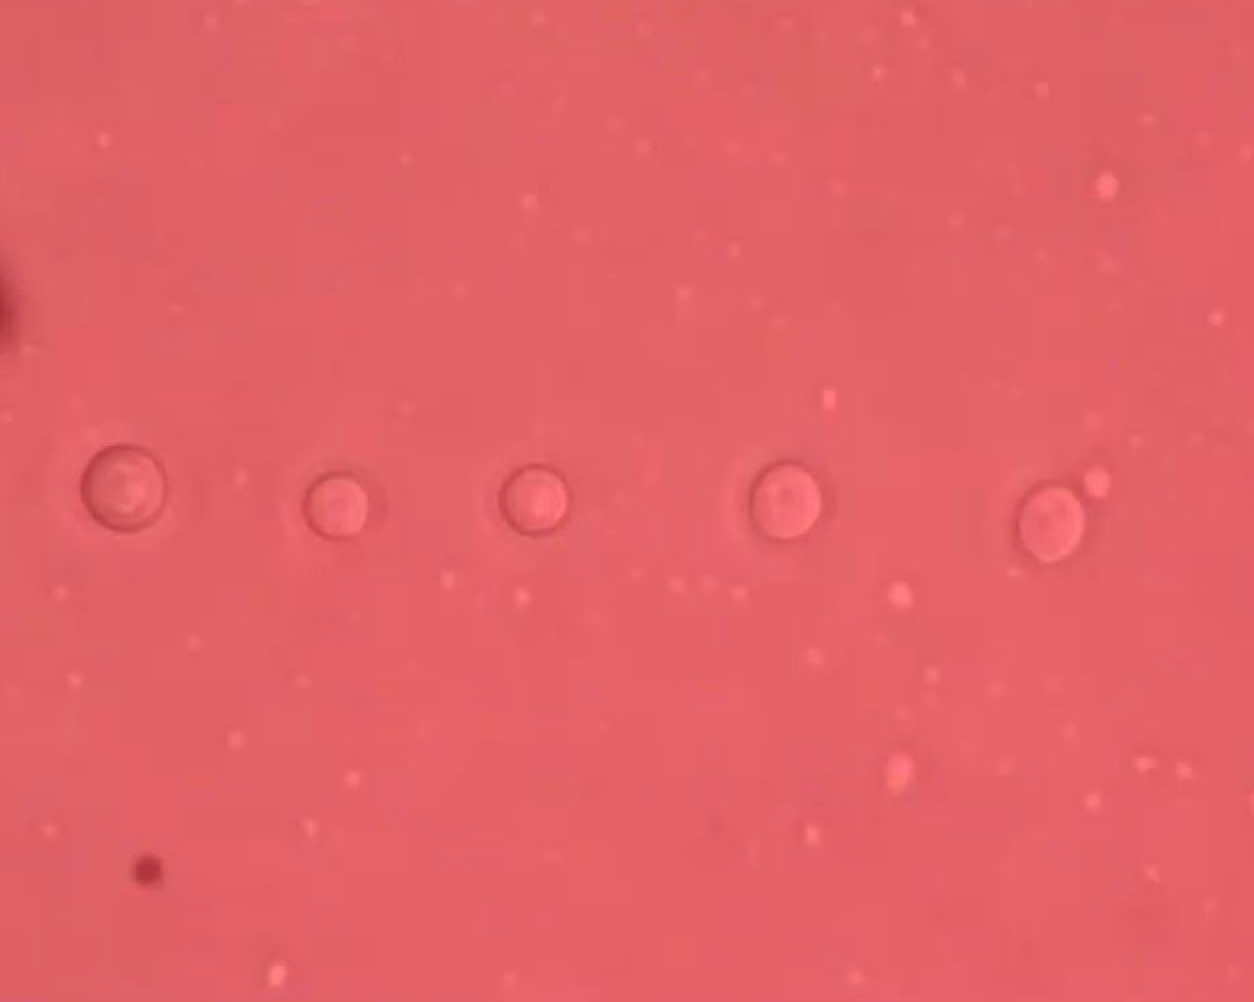
\includegraphics[width=\linewidth]{particlesnow.png} % Renombra tu archivo a este
    \caption*{\textbf{(c)}}
    \label{fig7:c}
  \end{subfigure}\hspace{0.5cm} % Espacio horizontal de 0.5cm
  \begin{subfigure}[b]{0.2\linewidth}
    \includegraphics[width=\linewidth]{Particles3.png} % Renombra tu archivo a este
    \caption*{\textbf{(d)}}
    \label{fig7:d}
  \end{subfigure}
  \captionsetup{labelformat = empty}
  \caption{\textbf{Figura 16: }
Atrapamiento de células de levadura con el objetivo de inmersión en agua, con una potencia láser de $14mW$ y un expansor de haz de 10x. }
  \label{poresfrustrules}
\end{figure}


}




\only<2>{\framesubtitle{Opticución de celula de levadura.}

\begin{figure}
     \centering
     \begin{subfigure}[b]{0.49\textwidth}
         \centering
         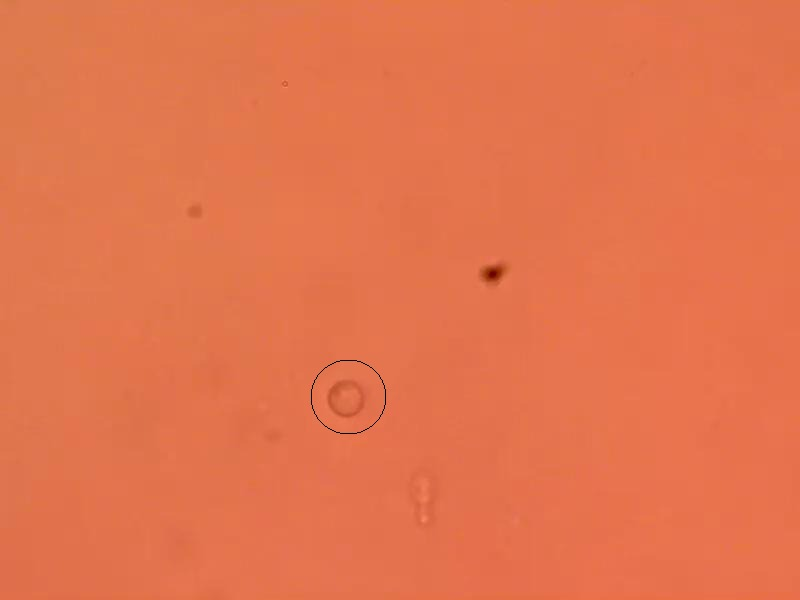
\includegraphics[width=0.50\textwidth]{Imagenes teoria/opticution0_edited.jpeg}
         \caption{Trapped yeast cell with 14 $mW$}
         \label{fig:y equals x}
     \end{subfigure}
     \hfill
     \begin{subfigure}[b]{0.49\textwidth}
         \centering
         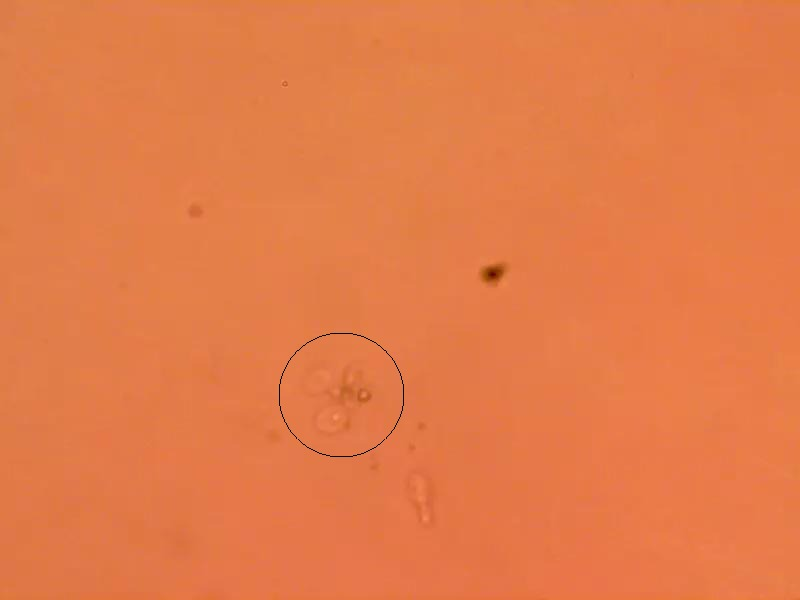
\includegraphics[width=0.50\textwidth]{Imagenes teoria/opticution1_edited.jpeg}
         \caption{Opticuted yeast cell with 695 $mW$}
         \label{fig:three sin x}
     \end{subfigure}
     \captionsetup{labelformat = empty}
     \caption{\textbf{Figura 17:} Opticución (muerte por luz) de una célula de levadura con un expansor de haz de 10x y el objetivo microscópico de inmersión en agua.
}
     \label{opticution}
     \hfill
\end{figure}

}
\end{frame}


\begin{frame}<1-4>
\frametitle{Resultados}\framesubtitle{Atrapamiento de diatomeas pennada}

\only<1>{

\begin{figure}
  \centering
  \begin{subfigure}[b]{0.2\linewidth}
    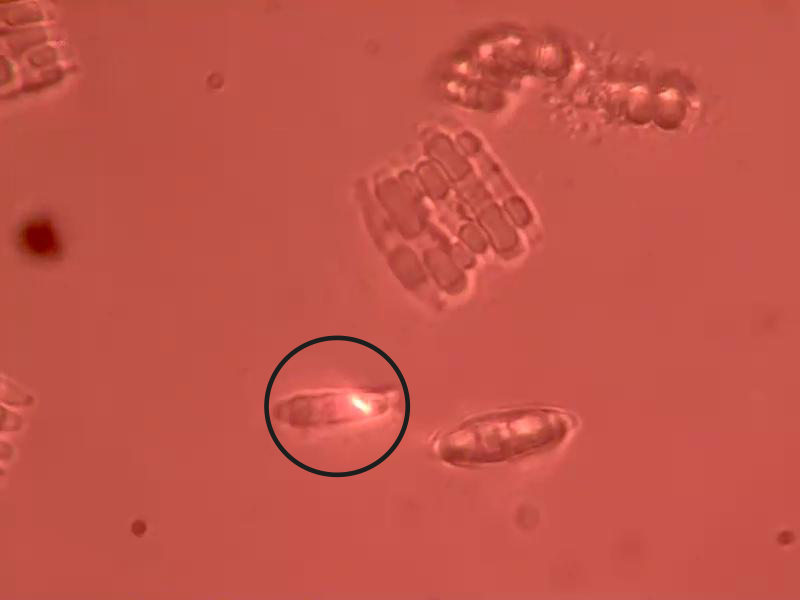
\includegraphics[width=\linewidth ,height=2.3cm]{ResultadosAlgea1/11.png} % Renombra tu archivo a este
    \caption*{\textbf{(a)}}
    \label{fig7:a}
    %\vspace{0.1cm}
  \end{subfigure}\hspace{0.5cm} % Espacio horizontal de 0.5cm
  \begin{subfigure}[b]{0.2\linewidth}
    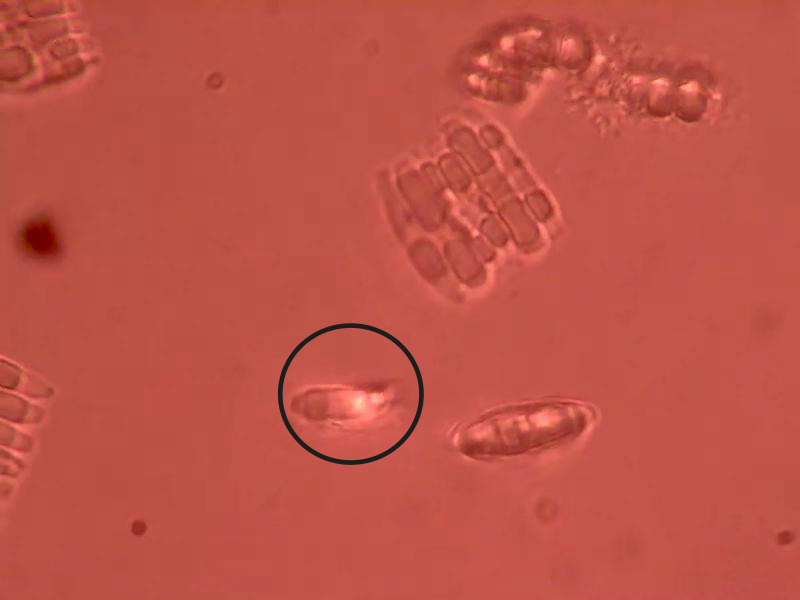
\includegraphics[width=\linewidth ,,height=2.3cm]{ResultadosAlgea1/levantando.png} % Renombra tu archivo a este
    \caption*{\textbf{(b)}}
    \label{fig7:b}
    %\vspace{0.2cm}
  \end{subfigure}

  \begin{subfigure}[b]{0.2\linewidth}
    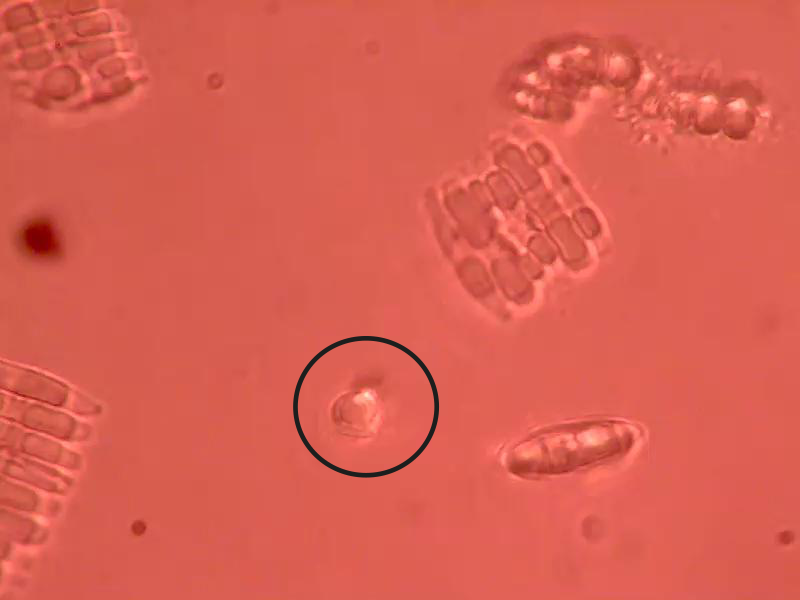
\includegraphics[width=\linewidth]{ResultadosAlgea1/3.png} % Renombra tu archivo a este
    \caption*{\textbf{(c)}}
    \label{fig7:c}
  \end{subfigure}\hspace{0.5cm} % Espacio horizontal de 0.5cm
  \begin{subfigure}[b]{0.2\linewidth}
    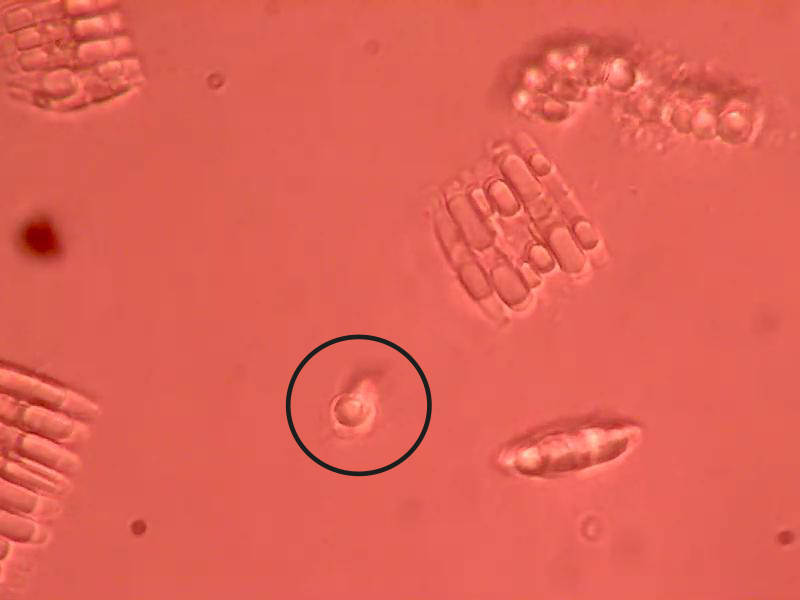
\includegraphics[width=\linewidth]{ResultadosAlgea1/1.png} % Renombra tu archivo a este
    \caption*{\textbf{(d)}}
    \label{fig7:d}
  \end{subfigure}
   \captionsetup{labelformat = empty}
  \caption{\textbf{Figura 18:} 
Manipulación de \textit{Nitzschia Sp.1} (pennada) con el objetivo de inmersión en agua (MO) y un expansor de haz de 10x. La potencia láser se estableció en 25 $mW$. (a-d) Cuadros del video grabado al someter la diatomea al haz láser: (a) Primero, la partícula se encuentra sobre la superficie del portaobjetos con el láser apagado. (b-c) Cuando se enciende el láser, la diatomea comienza a moverse hacia su posición de atrapamiento dentro de las pinzas ópticas (subfigura (d)) debido a la fuerza de gradiente. }
  \label{poresfrustrules}
\end{figure}


}

\only<2>{

\begin{figure}
  \centering
  \begin{subfigure}[b]{0.2\linewidth}
    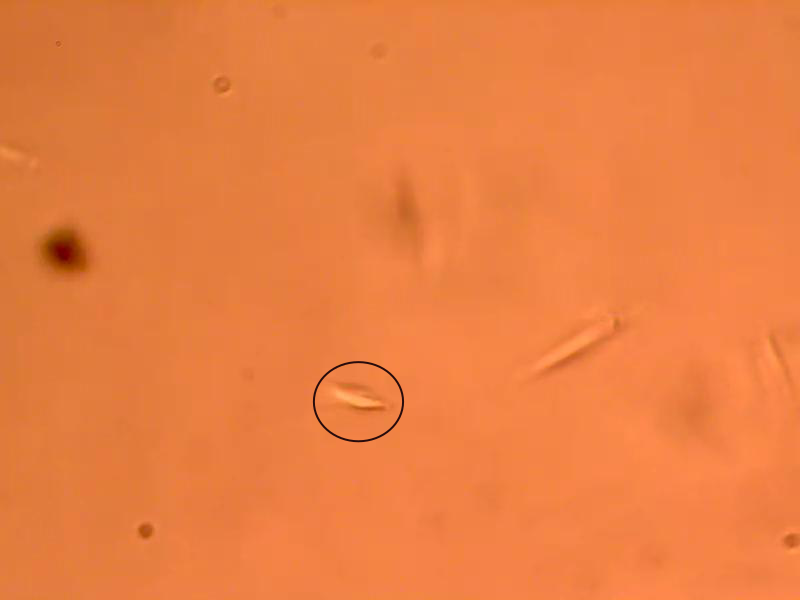
\includegraphics[width=\linewidth ,height=2.3cm]{Results/Resultadosalgea2/firstwatter secondalgea.png} % Renombra tu archivo a este
    \caption*{\textbf{(a)}}
    \label{fig7:a}
    %\vspace{0.1cm}
  \end{subfigure}\hspace{0.5cm} % Espacio horizontal de 0.5cm
  \begin{subfigure}[b]{0.2\linewidth}
    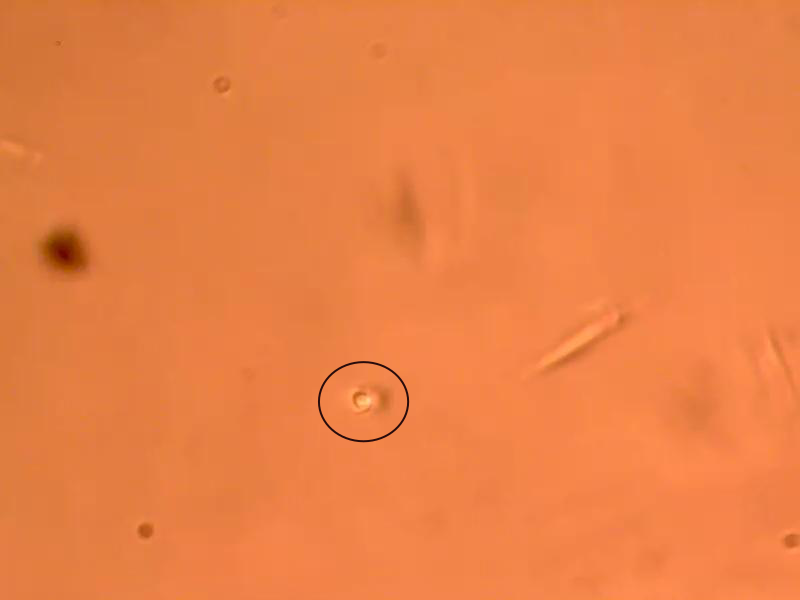
\includegraphics[width=\linewidth ,,height=2.3cm]{Results/Resultadosalgea2/secondalgea2water.png} % Renombra tu archivo a este
    \caption*{\textbf{(b)}}
    \label{fig7:b}
    %\vspace{0.2cm}
  \end{subfigure}

  \begin{subfigure}[b]{0.2\linewidth}
    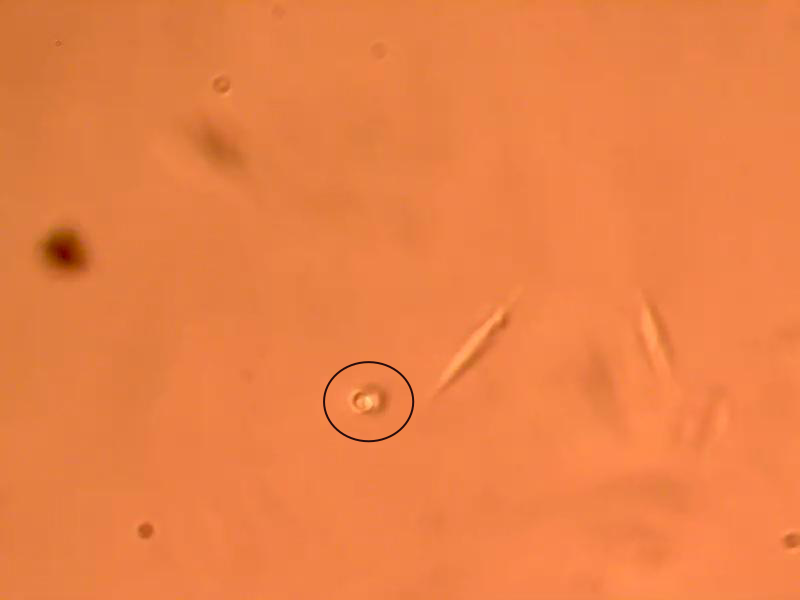
\includegraphics[width=\linewidth]{Results/Resultadosalgea2/secondalgeawater3.png} % Renombra tu archivo a este
    \caption*{\textbf{(c)}}
    \label{fig7:c}
  \end{subfigure}\hspace{0.5cm} % Espacio horizontal de 0.5cm
  \begin{subfigure}[b]{0.2\linewidth}
    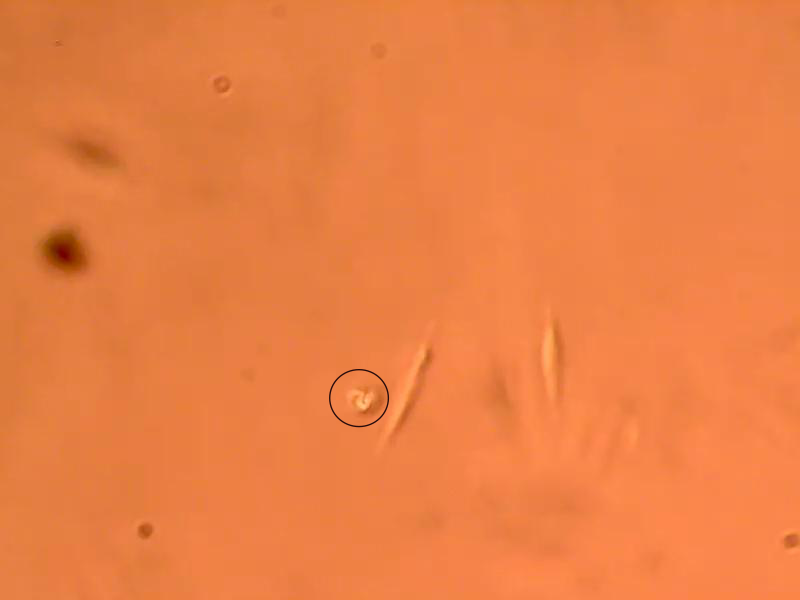
\includegraphics[width=\linewidth]{Results/Resultadosalgea2/secondalgeawater4.png} % Renombra tu archivo a este
    \caption*{\textbf{(d)}}
    \label{fig7:d}
  \end{subfigure}
   \captionsetup{labelformat = empty}
  \caption{\textbf{Figura 19: }
Atrapamiento de \textit{Phaeodactylum tricornutum} (pennada) con el objetivo de inmersión en agua (MO) y un expansor de haz de 10x. La potencia del láser se estableció en 19~mW. (a-d) Cuadros del video grabado al someter la diatomea al haz láser: (a) Primero, la partícula se encuentra sobre la superficie del portaobjetos con el láser apagado. (b-c) Cuando se enciende el láser, la diatomea comienza a desplazarse hacia su posición de atrapamiento dentro de las pinzas ópticas (subfigura (d)) debido a la fuerza de gradiente. }
  \label{poresfrustrules}
\end{figure}


}



\only<3>{

\begin{figure}
     \centering
     \begin{subfigure}[b]{0.3\textwidth}
         \centering
         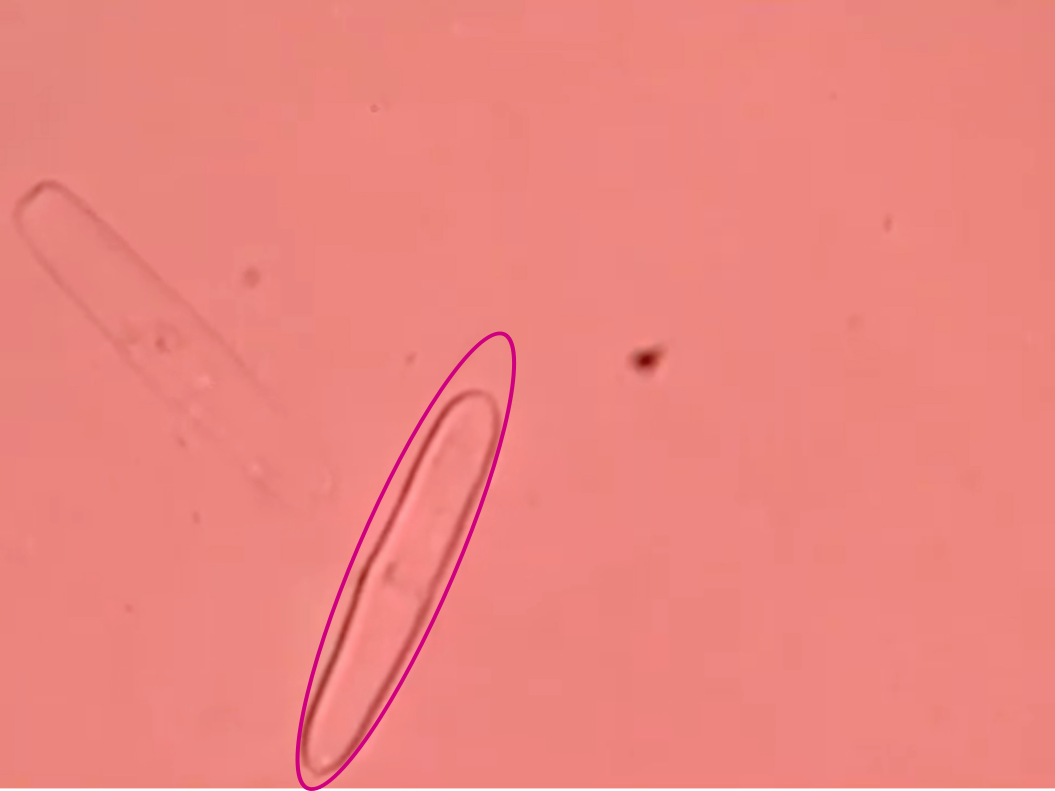
\includegraphics[width=\textwidth]{Results/Fifth/pennate1water.png}
         \caption{}
         \label{fig:y equals x}
     \end{subfigure}
     \hfill
     \begin{subfigure}[b]{0.3\textwidth}
         \centering
         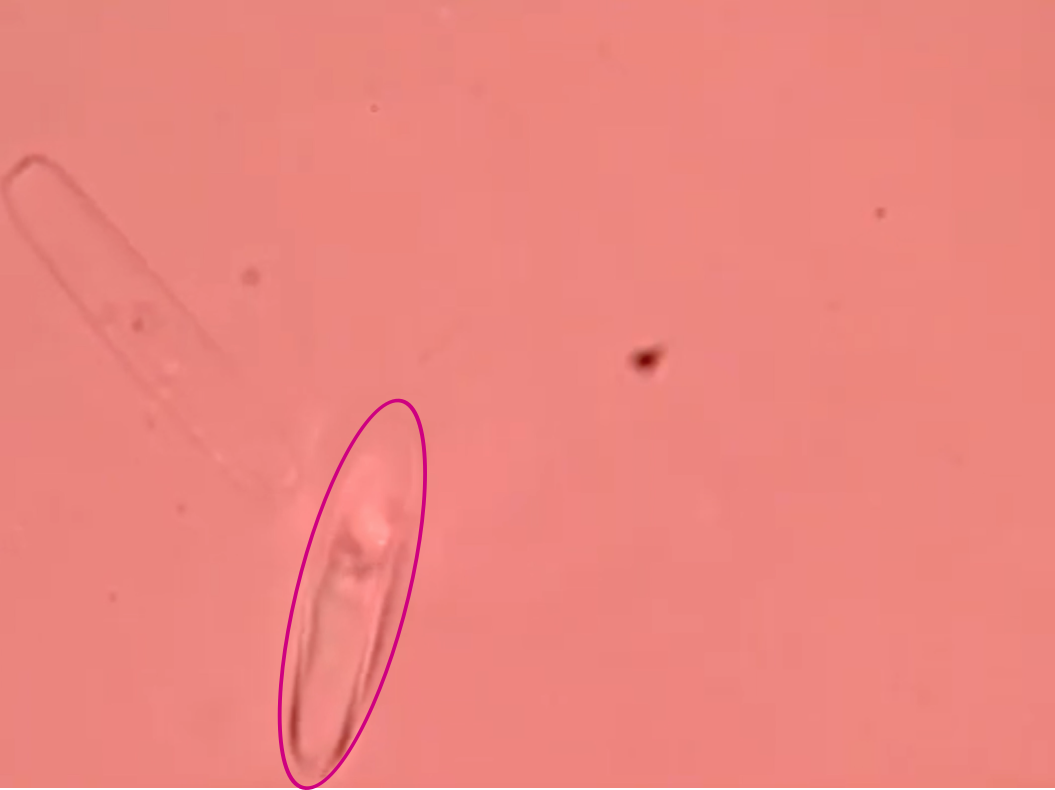
\includegraphics[width=\textwidth]{Results/Fifth/pennatewater2.png}
         \caption{}
         \label{fig:three sin x}
     \end{subfigure}
     \hfill
     \begin{subfigure}[b]{0.3\textwidth}
         \centering
         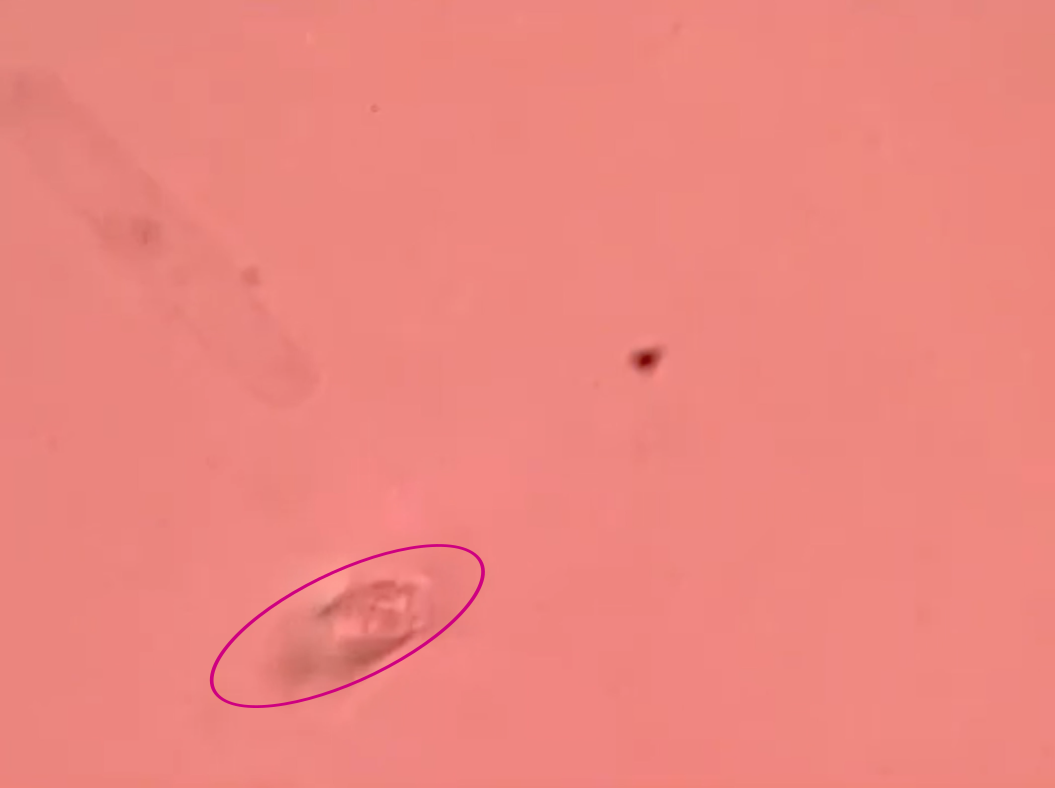
\includegraphics[width=\textwidth]{Results/Fifth/pennate3water.png}
         \caption{}
         \label{fig:five over x}
     \end{subfigure}
        \captionsetup{labelformat = empty}
     \caption{\textbf{Figura 20:} Atrapamiento de \textit{Marine pennada} (pennada) con el objetivo de inmersión en aceite (MO) y un expansor de haz de 2x. La potencia láser se estableció en 232 $mW$. (a-c) Cuadros ordenados cronológicamente del video grabado del atrapamiento de la diatomea pennada mencionada. (a) La diatomea comienza estando sobre la superficie del portaobjetos cuando el láser está apagado. (b-c) Cuando se enciende el láser, la diatomea se mueve hacia su posición de atrapamiento dentro de las pinzas ópticas debido a la fuerza de gradiente.}
\label{WIFORTH1}
     
\end{figure}

}

\only<4>{


\begin{figure}[H]
     \centering
     \begin{subfigure}[b]{0.3\textwidth}
         \centering
         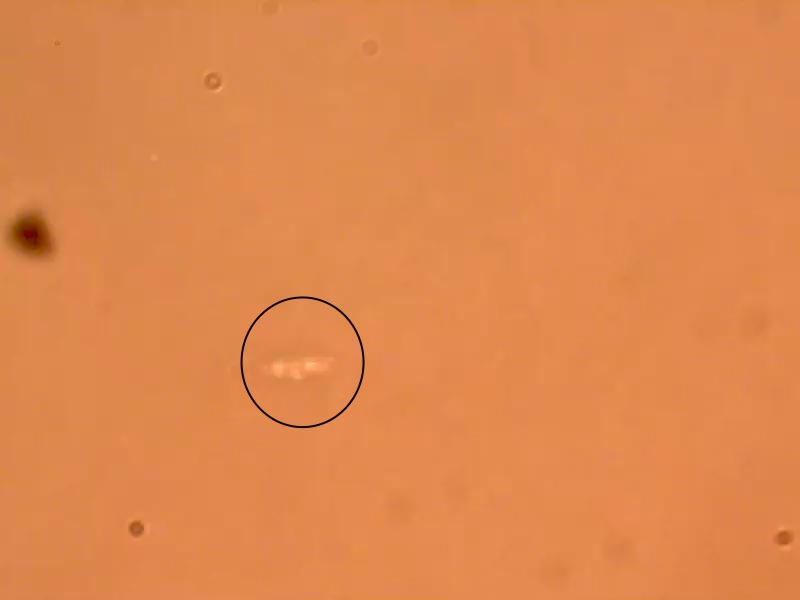
\includegraphics[width=\textwidth]{Results/Resultsforthalgae/falgae1_image2327.png}
         \caption{}
         \label{fig:y equals x}
     \end{subfigure}
     \hfill
     \begin{subfigure}[b]{0.3\textwidth}
         \centering
         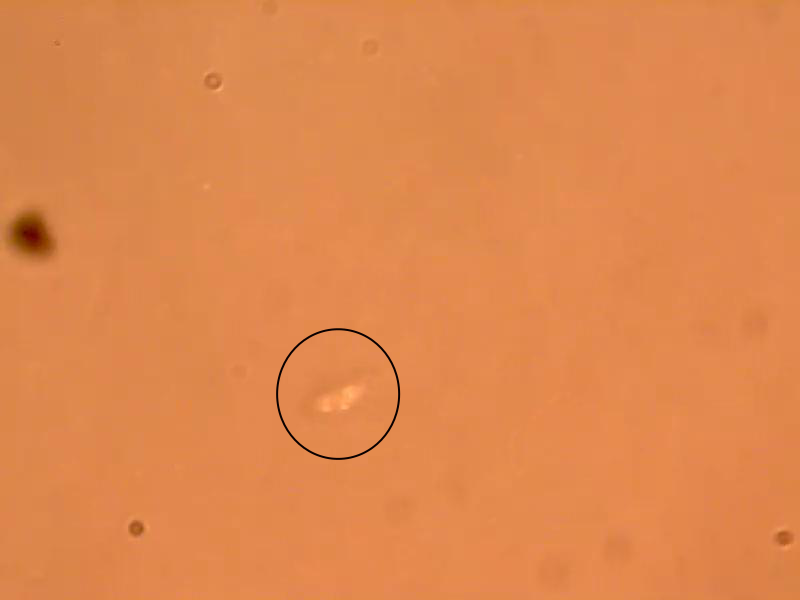
\includegraphics[width=\textwidth]{Results/Resultsforthalgae/falgae2.png}
         \caption{}
         \label{fig:three sin x}
     \end{subfigure}
     \hfill
     \begin{subfigure}[b]{0.3\textwidth}
         \centering
         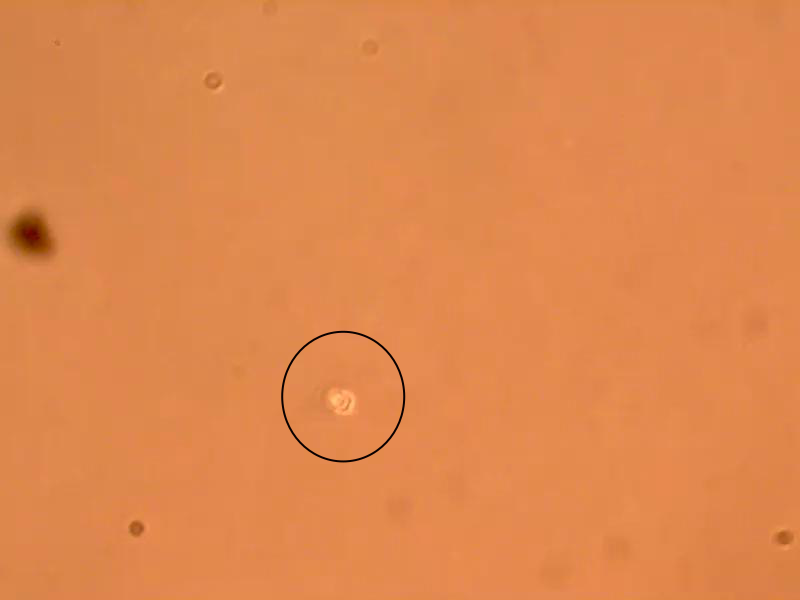
\includegraphics[width=\textwidth]{Results/Resultsforthalgae/falgae3.png}
         \caption{}
         \label{fig:five over x}
     \end{subfigure}
        \captionsetup{labelformat = empty}
     \caption{\textbf{Figura 21:} Atrapamiento de \textit{Navicula Sp.12} con el objetivo de inmersión en agua (MO) (pennada) y un expansor de haz de 10x. La potencia láser se estableció en 31 $mW$. (a-c) Cuadros ordenados cronológicamente del video grabado del atrapamiento de la diatomea \textit{Navicula Sp.12}. (a) La diatomea comienza estando sobre la superficie del portaobjetos cuando el láser está apagado. (b-c) Cuando se enciende el láser, la diatomea se mueve hacia su posición de atrapamiento dentro de las pinzas ópticas debido a la fuerza de gradiente.}
\label{WITHIRD1}
     
\end{figure}




}




\end{frame}

\begin{frame}<1>
\frametitle{Resultados}\framesubtitle{Atrapamiento de  diatomea céntrica}

\only<1>{


\begin{figure}
  \centering
  \begin{subfigure}[b]{0.2\linewidth}
    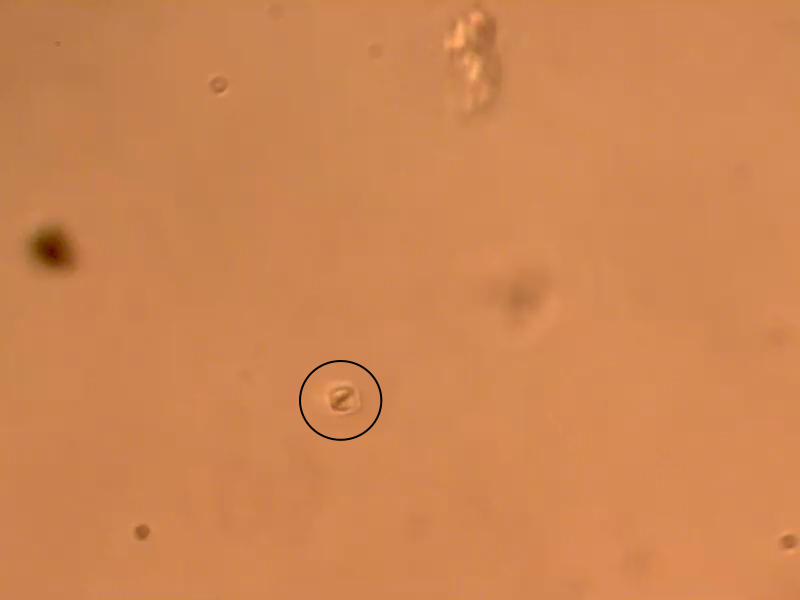
\includegraphics[width=\linewidth ,height=2.3cm]{Results/Pseudonana water/wpseudona1.png} % Renombra tu archivo a este
    \caption*{\textbf{(a)}}
    \label{fig7:a}
    %\vspace{0.1cm}
  \end{subfigure}\hspace{0.5cm} % Espacio horizontal de 0.5cm
  \begin{subfigure}[b]{0.2\linewidth}
    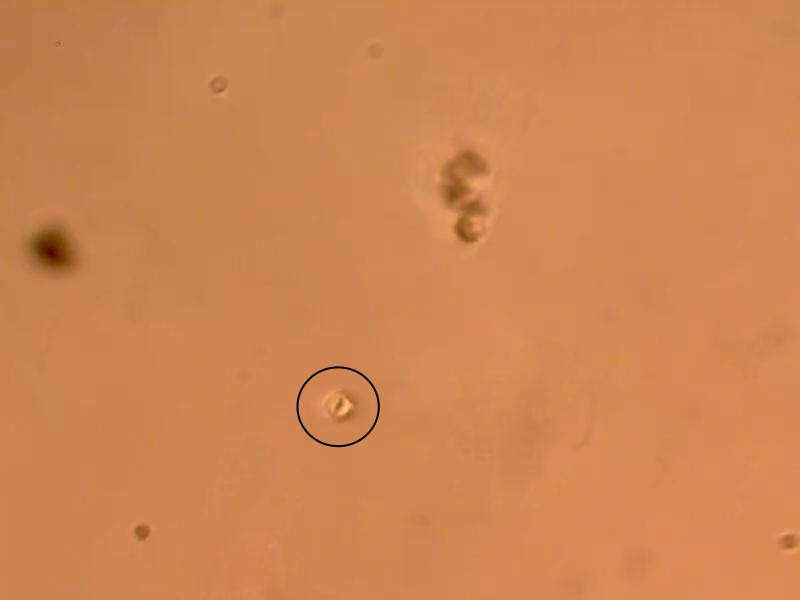
\includegraphics[width=\linewidth ,,height=2.3cm]{Results/Pseudonana water/wpseudonana2.png} % Renombra tu archivo a este
    \caption*{\textbf{(b)}}
    \label{fig7:b}
    %\vspace{0.2cm}
  \end{subfigure}

  \begin{subfigure}[b]{0.2\linewidth}
    \includegraphics[width=\linewidth]{Results/Pseudonana water/wpseudonana3.png} % Renombra tu archivo a este
    \caption*{\textbf{(c)}}
    \label{fig7:c}
  \end{subfigure}\hspace{0.5cm} % Espacio horizontal de 0.5cm
  \begin{subfigure}[b]{0.2\linewidth}
    \includegraphics[width=\linewidth]{Results/Pseudonana water/wpseudonana4.png} % Renombra tu archivo a este
    \caption*{\textbf{(d)}}
    \label{fig7:d}
  \end{subfigure}
   \captionsetup{labelformat = empty}
  \caption{\textbf{Figura 22: }
Atrapamiento de \textit{Thalassiosira pseudonana} (céntrica) con el objetivo de inmersión en agua (MO) y un expansor de haz de 10x. La potencia láser se estableció en 11 $mW$. (a-d) Cuadros del video grabado al someter la diatomea al haz láser: La partícula atrapada permanece inmóvil debido a la acción de la fuerza de gradiente, mientras que las partículas circundantes cambiaron su posición relativa. }
  \label{poresfrustrules}
\end{figure}

}



\end{frame}


\begin{frame}<1>
\frametitle{Results}\framesubtitle{Atrapamiento en microfluidicos}



\only<1>{\framesubtitle{Cálculo de fuerza gradiente}


\begin{figure}[H]
     \centering
     \begin{subfigure}[b]{0.49\textwidth}
         \centering         \includegraphics[width=0.95\textwidth]{Newplots_microfluidics_results/Force_silica_particle.png}
         %surpass the gradient force.
         \caption{Optical tweezers performance for the spherical 6.59 $\mu m$ $SiO_2$ particles.}
         \label{fig:yx}
     \end{subfigure}
     \hfill
     \begin{subfigure}[b]{0.49\textwidth}
         \centering
         \includegraphics[width=0.95\textwidth]{Newplots_microfluidics_results/Force_Thalassiosira.png}
         \caption{Optical tweezers performance for the \textit{Thalassiosira pseudonana} diatom.}
         \label{figx}
     \end{subfigure}
      \captionsetup{labelformat = empty}
     \caption{\textbf{Figura 23:} Fuerza de arrastre necesaria para superar la fuerza de gradiente de las pinzas ópticas para (a) partículas esféricas artificiales de sílice y (b) la diatomea \textit{Thalassiosira pseudonana}. El eje vertical representa la fuerza de Stokes para las diferentes potencias láser en el eje horizontal.}
     \hfill
    \label{forces_microfluidcs} 
\end{figure}



}


\end{frame}





\section{Conclusiones}
%-------------------------------------------------------
\begin{frame}<1-4>\frametitle{Conclusiones}
%-------------------------------------------------------
\only<1>{
\begin{itemize}
    \item \textbf{Primera parte – Manipulación de partículas artificiales:}
    \begin{itemize}
        \item Se usaron partículas de sílice esféricas (6.59 µm y 4.27 µm) para manipulación 3D.
        \item Partículas más grandes (19.98 µm y 24.82 µm) solo pudieron manipularse en 2D.
      %  \item Manipulación 3D de células de levadura, formando patrones sobre el portaobjetos.
       % \item Se observó muerte celular inducida por luz (\textit{opticution}) a diferentes potencias láser.
    \end{itemize}
\end{itemize}



}


\only<2>{



\begin{itemize}    
    \item \textbf{Segunda parte – Aplicación a organismos biológicos:}
    \begin{itemize}
            \item Manipulación 3D de células de levadura, formando patrones sobre el portaobjetos.
        \item Se observó muerte celular inducida por luz (\textit{opticution}).
        \item Manipulación de especies de diatomeas: \textit{Nitzchia sp.1}, \textit{Phaeodactylum tricornutum}, \textit{Navicula Sp.12}, \textit{Marine pennada} y \textit{Thalassiosira pseudonana}.
        %\item Diatomeas con simetría bilateral tendieron a rotar y alinear su eje con el eje vertical.
    \end{itemize}
    
    \item \textbf{Uso de dispositivos microfluídicos:}
    \begin{itemize}
        \item Medición de la velocidad del fluído necesaria para liberar partículas atrapadas.
        \item Cálculo de la fuerza de gradiente a partir de la fuerza de Stokes.
        %\item Fuerzas experimentales mayores que las teóricas, posibles causas:

    \end{itemize}
\end{itemize}





}


\only<3>{
Sobre la fuerza de Stokes y la diferencia entre la fuerza experimental y la te\'orica.
\begin{figure}[H]
    \centering
    \includegraphics[width=0.5\textwidth]{profile.png}
     \captionsetup{labelformat = empty}
    \caption{\textbf{Figura 24:} Perfil de velocidad de un fluído}
    \label{fig:etiqueta}
\end{figure}

\blfootnote{Fuente de la figura: (Reisfeld, 2023)}
}

\only<4>{
\begin{itemize}

    \item \textbf{Perspectivas futuras:}
    \begin{itemize}
        \item Estudios detallados de células individuales de diatomeas.
 
        \item Comparaciones con distintas longitudes de onda y aumentos.
        \item Estudio de reproducción al cambiar el medio durante el atrapamiento.
     
        \item Estudios espectroscópicos del frústulo para analizar su protección frente a luz UV.
    \end{itemize}
    \end{itemize}

}



\end{frame}

\appendix
\setcounter{framenumber}{0}
\begin{frame}
\frametitle{Referencias} % or "References", depending on your language

\small % or \footnotesize for more compact text

% Increase spacing between items
\setlength{\parskip}{6pt} % adds space between paragraphs
\setlength{\itemsep}{6pt} % not needed unless you're using itemize

\begin{flushleft}
Kepler, J. (1619). \textit{De Cometis Libelli III. Astronomicus ... Physicus ... Astrologicus}. De cometis libelli tres I. astronomicus.

Maxwell, J. C. (1865). VIII. A dynamical theory of the electromagnetic field. \textit{Philosophical Transactions of the Royal Society of London}, \textit{155}, 459–512.

Nichols, E. F., et al. (1901). A preliminary communication on the pressure of heat and light radiation. \textit{Physical Review (Series I)}, \textit{13}(5), 307.

% (...continue with rest of references)
Maiman, T. H. (1960). Stimulated optical radiation in ruby. *Nature*, *187*(4736), 493–494.

% Full authors: Theodore H. Maiman

Ashkin, A. (1970). Acceleration and trapping of particles by radiation pressure. *Physical Review Letters*, *24*(4), 156.

% Full authors: Arthur Ashkin

Ashkin, A., et al. (1986). Observation of a single-beam gradient force optical trap for dielectric particles. *Optics Letters*, *11*(5), 288–290.

% Full authors: Arthur Ashkin, James M. Dziedzic, John E. Bjorkholm, Steven Chu




\end{flushleft}
\end{frame}


\begin{frame}
\frametitle{Referencias}
\small
\setlength{\parskip}{6pt}

\begin{flushleft}
Yan, Y., et al. (2019). Two-million-year-old snapshots of atmospheric gases from Antarctic ice. *Nature*, *574*(7780), 663–666.

% Full authors: Yuzhen Yan, Michael L. Bender, Edward J. Brook, Heather M. Clifford, Preston C. Kemeny, Andrei V. Kurbatov, Sean Mackay, Paul A. Mayewski, Jessica Ng, Jeffrey P. Severinghaus, others

Aguirre, L. E., et al. (2018). Diatom frustules protect DNA from ultraviolet light. *Scientific Reports*, *8*(1), 5138.

% Full authors: Luis Ever Aguirre, Liangqi Ouyang, Anders Elfwing, Mikael Hedblom, Angela Wulff, Olle Inganäs

Callegari, A., et al. (2015). Computational toolbox for optical tweezers in geometrical optics. *Journal of the Optical Society of America B*, *32*(5), B11–B19.

% Full authors: Agnese Callegari, Mite Mijalkov, A. Burak Gököz, Giovanni Volpe

Pau, P. C. F., et al. (1990). Application of Stokes' law to ions in aqueous solution. *Journal of Physical Chemistry*, *94*(6), 2671–2679.

% Full authors: Paul Chi Fu Pau, J. O. Berg, W. G. McMillan

Round, F. E., et al. (1990). *Diatoms: Biology and morphology of the genera*. Cambridge University Press.

% Full authors: Frank Eric Round, Richard M. Crawford, David G. Mann

Jones, P. H., et al. (2015). *Optical tweezers: Principles and applications*. Cambridge University Press.
\end{flushleft}
\end{frame}

% Slide 3
\begin{frame}
\frametitle{Referencias}
\small



\setlength{\parskip}{6pt}

\begin{flushleft}

Pedreira, A. (2012). *Navicula pupula - 588*. Biodiversidad Virtual Mundo Microscópico. Retrieved June 18, 2023, from \url{https://www.biodiversidadvirtual.org/micro/Navicula-pupula-img588.html}

% Full authors: Antonio Pedreira

Diatoms of North America. (n.d.). *Pinnularia Ehrenb. 1843*. Retrieved May 12, 2023, from \url{https://diatoms.org/genera/pinnularia}

% Full authors: Diatoms of North America website

Olympus. (n.d.). *Olympus IX70 Fluorescence Microscope Cutaway Diagram*. Retrieved June 25, 2023, from \url{https://www.olympus-lifescience.com/en/microscope-resource/primer/techniques/fluorescence/ix70fluorescence/}

% Full authors: Olympus America, Inc., William K. Fester, Michael W. Davidson, Mortimer Abramowitz

Wanucha, G. (2012, November). The hidden life of ocean microbes. *Oceans at MIT*. MIT. Retrieved October 4, 2023, from \url{http://oceans.mit.edu/news/featured-stories/hidden-life-ocean-microbes.html}

% Full authors: Genevieve Wanucha

Reisfeld, B. (2021). *Fluids and Fluid Flow*. Retrieved from \url{https://www.engr.colostate.edu/CBE101/topics/fluids_and_fluid_flow.html}

% Full authors: Philip H. Jones, Onofrio M. Maragò, Giovanni Volpe


\end{flushleft}
\end{frame}

\begin{frame}
\frametitle{Referencias}
\small
\setlength{\parskip}{6pt}
\begin{flushleft}
Sonek, G. J., et al. (1994). Spectral fluorescence and scattering of cyanobacteria and diatoms held by optical tweezers. In Ocean Optics XII (Vol. 2258, pp. 568--574). SPIE.


Olof, S. N. et al. (2012). Measuring nanoscale forces with living probes. \textit{Nano letters}, \textit{12}(11), 6018--6023.
\end{flushleft}
\end{frame}



\end{document}
